\documentclass[12pt,a4paper]{report}

% Page Layout and Geometry
\usepackage[a4paper, top=1in, bottom=1in, left=1.2in, right=1in]{geometry}
\usepackage{setspace}
\onehalfspacing

% Typography and Encodings
\usepackage[utf8]{inputenc}
\usepackage[T1]{fontenc}
\usepackage{times}
\usepackage{microtype}

% Mathematical Formatting
\usepackage{amsmath, amssymb, amsfonts, amsthm}

% Tables and Visuals
\usepackage{booktabs}
\usepackage{multirow}
\usepackage{makecell}
\usepackage{tabularx}
\usepackage{graphicx}
\usepackage{float}
\graphicspath{{figures/}}

% TikZ and Diagramming
\usepackage{tikz}
\usetikzlibrary{shapes.geometric, arrows.meta, positioning, calc, fit, backgrounds}

% Algorithms and Pseudo-code
\usepackage{algorithm}
\usepackage{algpseudocode}

% Code Listings
\usepackage{listings}
\usepackage{xcolor}

\definecolor{codegreen}{rgb}{0,0.55,0.2}
\definecolor{codegray}{rgb}{0.45,0.45,0.45}
\definecolor{codepurple}{rgb}{0.55,0,0.75}
\definecolor{backcolour}{rgb}{0.97,0.97,0.98}
\definecolor{keywordblue}{rgb}{0.1,0.2,0.7}

\lstdefinestyle{mystyle}{
    backgroundcolor=\color{backcolour},   
    commentstyle=\color{codegreen}\itshape,
    keywordstyle=\color{keywordblue}\bfseries,
    numberstyle=\tiny\color{codegray},
    stringstyle=\color{codepurple},
    basicstyle=\ttfamily\footnotesize,
    breakatwhitespace=false,         
    breaklines=true,                 
    captionpos=b,                    
    keepspaces=true,                 
    numbers=left,                    
    numbersep=6pt,                  
    showspaces=false,                
    showstringspaces=false,
    showtabs=false,                  
    tabsize=4,
    frame=single,
    rulecolor=\color{black!20},
    xleftmargin=10pt,
    xrightmargin=5pt
}
\lstset{style=mystyle}

% Section Heading Formatting (16, 14, 12 Rule)
\usepackage{titlesec}
\titleformat{\chapter}[display]
  {\normalfont\fontsize{18}{22}\bfseries}{\chaptertitlename\ \thechapter}{14pt}{\fontsize{18}{22}\bfseries}
\titleformat{\section}
  {\normalfont\fontsize{15}{18}\bfseries}{\thesection}{1em}{}
\titleformat{\subsection}
  {\normalfont\fontsize{13}{16}\bfseries}{\thesubsection}{1em}{}
\titleformat{\subsubsection}
  {\normalfont\fontsize{12}{15}\bfseries}{\thesubsubsection}{1em}{}

% Hyperlinks
\usepackage{hyperref}
\hypersetup{
    colorlinks=true,
    linkcolor=blue!75!black,
    citecolor=green!50!black,
    urlcolor=purple!70!black,
    pdfauthor={Venkata Dhanush K., Veera Nidhish G., Settipalli Raja Rushi Praneeth R., Evvala Venkata Lakshmi Narasimha V.},
    pdftitle={Deep Semantic Sequence Modeling and Lightweight Optimization for Robust Syslog Anomaly Detection},
    pdfsubject={Final Year Capstone Project Report},
    pdfkeywords={Log Anomaly Detection, Syslog, Autoencoder, Word2Vec, Extreme Value Theory, Peaks-Over-Threshold}
}

\begin{document}

% -------------------------------------------------------------
% FRONT MATTER
% -------------------------------------------------------------
\pagenumbering{roman}

% Title Page
\begin{titlepage}
    \centering
    \vspace*{0.5cm}
    
    {\Large\bfseries VIT-AP UNIVERSITY\par}
    {\large Near Vijayawada, Amaravati, Andhra Pradesh -- 522237, India\par}
    {\large\bfseries School of Computer Science and Engineering\par}
    
    \vspace{1.5cm}
    
    \begin{center}
        \rule{0.8\textwidth}{1.2pt}\\[0.4cm]
        {\LARGE\bfseries Deep Semantic Sequence Modeling and Lightweight Optimization for Robust Syslog Anomaly Detection\par}
        \vspace{0.2cm}
        {\large\itshape Final Year Capstone Project Report\par}
        \rule{0.8\textwidth}{1.2pt}
    \end{center}
    
    \vspace{0.8cm}
    
    {\small\textbf{Project Specialization:}\par}
    {\normalsize System Software, Distributed Systems, and Machine Learning\par}
    
    \vspace{1.5cm}
    
    {\large\bfseries Submitted by:\par}
    \vspace{0.4cm}
    \begin{tabular}{ll}
        \textbf{Venkata Dhanush Kakarlamudi} & (Reg. No.: 23BCE8172) \\
        \textbf{Veera Nidhish Gondimalla} & (Reg. No.: 23BCE7421) \\
        \textbf{Settipalli Raja Rushi Praneeth Reddy} & (Reg. No.: 23BCE7425) \\
        \textbf{Evvala Venkata Lakshmi Narasimha Veereswar} & (Reg. No.: 23BCE7439) \\
    \end{tabular}
    
    \vspace{1.5cm}
    
    {\normalsize\itshape In partial fulfillment for the award of the degree of\par}
    \vspace{0.2cm}
    {\large\bfseries BACHELOR OF TECHNOLOGY\par}
    {\normalsize in\par}
    {\large\bfseries COMPUTER SCIENCE AND ENGINEERING\par}
    
    \vfill
    
    {\large\bfseries Academic Year: 2026--2027\par}
    {\normalsize Date of Submission: November 2026\par}
\end{titlepage}


\cleardoublepage

% Certificate Placeholder
\chapter*{Certificate}
\addcontentsline{toc}{chapter}{Certificate}

\noindent This is to certify that the project report entitled \textbf{``Deep Semantic Sequence Modeling and Lightweight Optimization for Robust Syslog Anomaly Detection''}, submitted by:

\begin{itemize}
    \item \textbf{Venkata Dhanush Kakarlamudi} (Register No: 23BCE8172)
    \item \textbf{Veera Nidhish Gondimalla} (Register No: 23BCE7421)
    \item \textbf{Settipalli Raja Rushi Praneeth Reddy} (Register No: 23BCE7425)
    \item \textbf{Evvala Venkata Lakshmi Narasimha Veereswar} (Register No: 23BCE7439)
\end{itemize}

\noindent in partial fulfillment for the award of the degree of \textbf{Bachelor of Technology in Computer Science and Engineering} at \textbf{VIT-AP University, Amaravati}, is a bonafide record of original work carried out by them under my supervision and guidance during the academic year 2026--2027.

\noindent The results embodied in this report have not been submitted to any other university or institute for the award of any degree or diploma.

\vspace{3.0cm}

\noindent
\begin{minipage}{0.45\textwidth}
    \centering
    \textbf{Project Supervisor} \\
    School of Computer Science and Engineering \\
    VIT-AP University, Amaravati
\end{minipage}
\hfill
\begin{minipage}{0.45\textwidth}
    \centering
    \textbf{Dean / Head of the Department} \\
    School of Computer Science and Engineering \\
    VIT-AP University, Amaravati
\end{minipage}

\vspace{2.0cm}

\noindent \textbf{Internal Examiner} \hfill \textbf{External Examiner}


\cleardoublepage

% Declaration Placeholder
\chapter*{Declaration}
\addcontentsline{toc}{chapter}{Declaration}

\noindent We hereby declare that the capstone project work entitled \textbf{``Deep Semantic Sequence Modeling and Lightweight Optimization for Robust Syslog Anomaly Detection''} is an authentic record of our own research and engineering work conducted at the School of Computer Science and Engineering, VIT-AP University, Amaravati.

\noindent We confirm that:
\begin{enumerate}
    \item The work presented herein is original and has been completed under the strict ethical and empirical guidelines set forth by the institution.
    \item All numerical evaluations, model metrics, hardware measurements, and baseline comparisons are fully reproducible from the provided source artifacts without artificial data manipulation.
    \item Any material, algorithm, theoretical formulation, or literature previously published by other researchers has been duly acknowledged, cited, and referenced in accordance with standard academic integrity practices.
    \item This document has not been submitted in part or full for the award of any other academic degree, diploma, or certificate at this or any other institution.
\end{enumerate}

\vspace{2.5cm}

\noindent
\begin{minipage}{0.45\textwidth}
    \centering
    \textbf{Venkata Dhanush Kakarlamudi}\\
    (23BCE8172)
\end{minipage}
\hfill
\begin{minipage}{0.45\textwidth}
    \centering
    \textbf{Veera Nidhish Gondimalla}\\
    (23BCE7421)
\end{minipage}

\vspace{1.8cm}

\noindent
\begin{minipage}{0.45\textwidth}
    \centering
    \textbf{Settipalli Raja Rushi Praneeth Reddy}\\
    (23BCE7425)
\end{minipage}
\hfill
\begin{minipage}{0.45\textwidth}
    \centering
    \textbf{Evvala Venkata Lakshmi Narasimha Veereswar}\\
    (23BCE7439)
\end{minipage}

\vspace{2.0cm}

\noindent \textbf{Place:} Amaravati, Andhra Pradesh \\
\textbf{Date:} November 17, 2026


\cleardoublepage

% Acknowledgements
\chapter*{Acknowledgements}
\addcontentsline{toc}{chapter}{Acknowledgements}

We would like to express our deep sense of gratitude and profound respect to our project supervisor for their invaluable guidance, constructive criticism, and relentless encouragement throughout the duration of this capstone research project. Their deep insights into machine learning systems, statistical modeling, and empirical rigor have been instrumental in shaping the methodology and scientific standards of this work.

We extend our sincere thanks to the Management and Leadership of \textbf{VIT-AP University}, particularly the Dean and the faculty members of the \textbf{School of Computer Science and Engineering (SCOPE)}, for providing the state-of-the-art computational facilities, continuous institutional support, and an intellectually stimulating academic environment.

We are immensely thankful to the global open-source and systems research communities, particularly the creators of the \textbf{LogHub} dataset repository and the authors of foundational baseline papers, whose benchmarks made this empirical investigation possible. 

Finally, we express our heartfelt appreciation to our parents, family members, and peers for their unwavering patience, encouragement, and moral support during the intensive phases of experimentation, debugging, and manuscript drafting.

\vspace{2.5cm}

\noindent \textbf{Venkata Dhanush Kakarlamudi} \\
\textbf{Veera Nidhish Gondimalla} \\
\textbf{Settipalli Raja Rushi Praneeth Reddy} \\
\textbf{Evvala Venkata Lakshmi Narasimha Veereswar}


\cleardoublepage

% Abstract
\chapter*{Abstract}
\addcontentsline{toc}{chapter}{Abstract}

System log streams represent the primary telemetry modality for tracking operational health, service reliability, and security integrity in large-scale distributed computing environments and mission-critical networked infrastructures. Modern telemetry streams generate millions of semi-structured log events across massively parallel nodes, making manual diagnostic inspection impossible and demanding automated, real-time anomaly detection pipelines. 

In this capstone research project, we present an exhaustive empirical investigation into the spectrum of log anomaly detection architectures, spanning lightweight linear subspace projections, robust decomposition techniques, and deep semantic reconstruction models. We begin by reproducing the foundational linear baselines established in recent literature (F{\"a}lt et al., IEEE ICSRS 2025) on the structured Hadoop Distributed File System (\textbf{HDFS\_v1}) benchmark (575,061 total blocks, 16,838 anomalous). Under the standard 5-fold cross-validation protocol (25,000 normal and 1,000 anomalous traces; 5,000 normals for fitting), we uncover that an undocumented $L_2$-normalization of raw event count vectors is strictly required to reproduce the published Principal Component Analysis (PCA, $k=6$) ceiling: our implementation achieves $94.60\%$ $F_1$-score, matching the reported $94.64\%$. Furthermore, replacing the literature's test-set oracle percentile cutoff with label-free Extreme Value Theory Peaks-Over-Threshold (POT) thresholding yields $95.95\% \pm 1.47\%$ $F_1$, successfully eliminating test-set leakage while remaining within statistical baseline noise. Conversely, extensive evaluation over 30 random seeds demonstrates that the published Robust PCA (RPCA) claim of $90.55\%$ $F_1$ is irreproducible under strict evaluation protocols (peaking at $87.38\%$), as clean training partitions cause low-rank matrix collapse to rank-2.

Crucially, when extending linear count-based models to the highly interleaved Blue Gene/L (\textbf{BGL}) supercomputing dataset (4,747,963 log lines, 1,848 Drain templates), linear models hit a strict mathematical ceiling of $\sim 65\%$ $F_1$. To overcome this barrier, we engineer a spatial-temporal sequence architecture that groups logs by physical node identity over 6-hour windows (yielding 1,286,817 sequences), projects events into continuous vector spaces via unsupervised Skip-Gram Word2Vec (32-d), aggregates representations using concatenated Mean + Max dual pooling ($z \in \mathbb{R}^{64}$), and reconstructs features through a deep Multi-Layer Perceptron (MLP) Autoencoder ($64 \rightarrow 32 \rightarrow 16 \rightarrow 32 \rightarrow 64$).

To establish unquestionable scientific rigor, we deploy a leak-free 10-fold cross-validation protocol under natural operating prevalence ($10.07\%$ anomalies, where every anomaly is tested exactly once and models are trained strictly on healthy behavior with zero test-label feedback). Under pure unsupervised EVT/POT thresholding on validation normal reconstruction errors (\textbf{Mode A}, headline result, $q=0.90$, target $\text{FPR}=10^{-3}$, $0/10$ fallbacks triggered), our system attains:
\begin{itemize}
    \item \textbf{Precision:} $93.76\% \pm 2.54\%$
    \item \textbf{Recall:} $82.61\% \pm 1.96\%$
    \item \textbf{F1-Score:} $\mathbf{87.80\% \pm 1.31\%}$
\end{itemize}
Under semi-supervised validation tuning (\textbf{Mode B}), the system attains Precision $93.06\% \pm 2.59\%$, Recall $84.71\% \pm 1.19\%$, and $F_1$-score $\mathbf{88.66\% \pm 1.07\%}$. Threshold-free ranking metrics confirm exceptional discriminative power, achieving Precision-Recall AUC of $\mathbf{91.05\% \pm 0.32\%}$ and ROC-AUC of $\mathbf{97.34\% \pm 0.15\%}$.

We definitively deconstruct earlier literature claims of $\sim 90.44\%$ $F_1$ by evaluating our exact trained models on an artificially balanced test set ($50\%$ anomalies): our models score $\mathbf{90.16\%}$ (Mode A) and $\mathbf{91.36\%}$ (Mode B) $F_1$. We prove that the gap between $87.80\%$ and $90.44\%$ is fundamentally driven by base-rate prevalence and test contamination in legacy scripts rather than algorithmic regression. Architectural ablations demonstrate that the non-linear Autoencoder significantly outperforms linear PCA ($59.97\%$ Mode A $F_1$) and Isolation Forest ($2.07\%$ Mode A $F_1$).

Furthermore, temporal robustness tests across a 70/10/20 chronological split expose a critical production challenge: Mode A $F_1$ collapses to $0.03\%$ due to severe concept drift and an Out-of-Vocabulary (OOV) token rate of $68.91\%$, proving that static embeddings cannot survive system evolution without periodic retraining. Finally, hardware benchmarks on an Apple M2 CPU reveal that the serialized autoencoder requires only \textbf{5,328 parameters} ($70.25\text{ KB}$ footprint), achieves a single-window latency of \textbf{43.2 microseconds} (batch latency $0.37\text{ }\mu\text{s/window}$), and delivers an end-to-end throughput of \textbf{62,076 windows/second} without GPU acceleration. We synthesize these empirical discoveries into a universal \textit{Dataset-Dependency Rule} governing telemetry anomaly detection systems.

\vspace{0.8cm}
\noindent\textbf{Keywords:} Log Anomaly Detection, System Telemetry, Autoencoder, Word2Vec, Extreme Value Theory, Peaks-Over-Threshold, Base-Rate Prevalence, Model Efficiency.


\cleardoublepage

% Table of Contents
\tableofcontents
\cleardoublepage

% List of Figures
\listoffigures
\addcontentsline{toc}{chapter}{List of Figures}
\cleardoublepage

% List of Tables
\listoftables
\addcontentsline{toc}{chapter}{List of Tables}
\cleardoublepage

% List of Abbreviations
\chapter*{List of Abbreviations}
\addcontentsline{toc}{chapter}{List of Abbreviations}

\begin{tabular}{ll}
\textbf{AE} & Autoencoder \\
\textbf{ALM} & Augmented Lagrange Multiplier \\
\textbf{AUC} & Area Under the Curve \\
\textbf{BGL} & Blue Gene/L Supercomputer (Lawrence Livermore National Laboratory) \\
\textbf{BPE} & Byte-Pair Encoding \\
\textbf{CapEx} & Capital Expenditure \\
\textbf{CPU} & Central Processing Unit \\
\textbf{CV} & Cross-Validation \\
\textbf{Drain} & Fixed-Depth Tree-based Online Log Parsing Algorithm \\
\textbf{EVT} & Extreme Value Theory \\
\textbf{FAR} & False Alarm Rate \\
\textbf{FN} & False Negative \\
\textbf{FP} & False Positive \\
\textbf{FPR} & False Positive Rate \\
\textbf{GPD} & Generalized Pareto Distribution \\
\textbf{GPU} & Graphics Processing Unit \\
\textbf{HDFS} & Hadoop Distributed File System \\
\textbf{ICSRS} & International Conference on System Reliability and Safety \\
\textbf{IDF} & Inverse Document Frequency \\
\textbf{IF} & Isolation Forest \\
\textbf{KDE} & Kernel Density Estimation \\
\textbf{LLM} & Large Language Model \\
\textbf{MLP} & Multi-Layer Perceptron \\
\textbf{NLP} & Natural Language Processing \\
\textbf{OOV} & Out-of-Vocabulary \\
\textbf{OpEx} & Operational Expenditure \\
\textbf{PCA} & Principal Component Analysis \\
\textbf{POT} & Peaks-Over-Threshold \\
\textbf{PR-AUC} & Precision-Recall Area Under the Curve \\
\textbf{ROC-AUC} & Receiver Operating Characteristic Area Under the Curve \\
\textbf{RPCA} & Robust Principal Component Analysis \\
\textbf{SVD} & Singular Value Decomposition \\
\textbf{TF-IDF} & Term Frequency - Inverse Document Frequency \\
\textbf{TN} & True Negative \\
\textbf{TP} & True Positive \\
\textbf{Word2Vec} & Continuous Distributed Vector Representation of Words/Tokens \\
\end{tabular}


\cleardoublepage

% -------------------------------------------------------------
% MAIN BODY CHAPTERS
% -------------------------------------------------------------
\pagenumbering{arabic}
\setcounter{page}{1}

% Chapter 1: Introduction
\chapter{Introduction}
\label{ch:intro}

\section{Context and Motivation}
\label{sec:intro_context}
In the contemporary landscape of computing, distributed systems, high-performance computing (HPC) clusters, cloud microservices, and enterprise server telemetry infrastructures have reached unprecedented scales of complexity. Modern data centers and distributed software stacks execute millions of concurrent threads across tens of thousands of heterogeneous compute nodes. In such massive environments, runtime component failures, network partitioning, distributed deadlocks, memory leaks, and malicious security breaches are not rare anomalies; they are inevitable operational certainties.

To maintain service level agreements (SLAs), guarantee high availability, and prevent cascading system outages, site reliability engineers (SREs) and operations teams rely heavily on \textbf{system telemetry logs} (syslogs). System logs are ubiquitous, append-only, semi-structured console messages emitted by operating systems, daemons, background services, network interfaces, and user-space applications. Every individual log entry records an instantaneous snapshot of system state, typically comprising a timestamp, hostname or node identifier, severity facility level (e.g., \texttt{INFO}, \texttt{WARNING}, \texttt{ERROR}, \texttt{FATAL}), and an unconstrained natural language textual narrative (e.g., \texttt{"Packet responder 10.0.1.4 timed out after 3000ms"}).

Because logs are generated autonomously without modifying source code or attaching runtime debuggers, they constitute the single most comprehensive and granular diagnostic window into the execution flow of production systems. However, the sheer volume of generated telemetry poses an existential challenge to manual inspection. A modern supercomputer or enterprise cloud cluster routinely produces hundreds of gigabytes of unstructured log text per day—amounting to millions of lines per hour. Human operators cannot manually read or parse this deluge of text to identify root causes. Consequently, there is an urgent and critical demand for automated, highly scalable, and accurate \textbf{log anomaly detection systems} capable of streaming analysis and real-time operational alerting.

\section{The Challenge of Log Anomaly Detection}
\label{sec:intro_challenges}
While anomaly detection is an established sub-field of machine learning, system logs introduce idiosyncratic domain-specific complexities that cause conventional statistical and tabular anomaly detection algorithms to fail:

\begin{enumerate}
    \item \textbf{Unstructured Free-Text Heterogeneity:} Unlike structured numeric metrics (such as CPU utilization percentage or memory consumption), log messages are written by human software developers using arbitrary strings, dynamic variables, IP addresses, hexadecimal memory offsets, and variable parameter values. There is no predefined database schema.
    \item \textbf{High-Volume Streaming and Computational Constraints:} Production monitoring systems operate under severe latency constraints. Telemetry pipelines must ingest, parse, vectorize, and evaluate hundreds of thousands of events per second. Detection pipelines that require computationally heavy deep neural networks, such as multi-layer bidirectional transformers, often incur prohibitively high inference latencies and multi-kilowatt power overheads, rendering edge deployment or localized node monitoring financially and computationally non-viable.
    \item \textbf{Multi-Tenant Concurrency and Asynchronous Interleaving:} In large-scale computing platforms—such as the Blue Gene/L supercomputer with 131,072 processing cores—thousands of independent tasks execute simultaneously. Log messages emitted by distinct nodes, parallel jobs, and system daemons are asynchronously funneled into centralized logging daemons, resulting in an intricately interleaved ``chronological soup'' where sequential dependencies between adjacent lines are severely corrupted.
    \item \textbf{Extreme Class Imbalance and Base-Rate Reality:} Anomalous behavior in well-engineered enterprise systems is rare. In natural operational settings, healthy sequences constitute $90\%$ to $99\%$ of all observations. Machine learning models trained on artificially balanced benchmarks frequently experience the catastrophic ``base-rate fallacy'' when deployed in production, where minor false positive rates unleash an overwhelming flood of false alarms, causing alert fatigue among human operators.
    \item \textbf{Continuous Software Evolution and Semantic Drift:} Software is dynamic. Kernel patches, application updates, and scheduled maintenance periodically introduce previously unseen log templates. Static machine learning models that lack mechanisms to handle out-of-vocabulary events quickly suffer from performance degradation when encountering evolving log distributions.
\end{enumerate}

\section{Research Objectives and Scope}
\label{sec:intro_objectives}
This capstone research project investigates the entire spectrum of log anomaly detection architectures, spanning classical lightweight linear subspace decomposition techniques, robust matrix formulation, continuous natural language embeddings, and non-linear deep neural autoencoders. Rather than treating published literature as unassailable truth, this work adopts a rigorously empirical, reproducible methodology designed to validate, critique, and extend recent findings in the field.

The specific objectives of this capstone research are defined as follows:

\begin{enumerate}
    \item \textbf{Rigorous Baseline Reproduction:} Conduct an exhaustive replication of the linear baseline models proposed in the 2025 IEEE International Conference on System Reliability and Safety (ICSRS) study by F{\"a}lt et al.~\cite{falt2025lightweight} on the structured Hadoop Distributed File System (\textbf{HDFS\_v1}) benchmark. Determine the precise mathematical and preprocessing conditions required to reproduce published Principal Component Analysis (PCA) and Robust Principal Component Analysis (RPCA) results.
    \item \textbf{Algorithmic Discovery of Undocumented Preprocessing:} Identify the hidden failure modes of raw count and TF-IDF representations, and formulate the exact geometric normalization required for linear subspace projection to succeed on structured session data.
    \item \textbf{Mathematical Investigation of the RPCA Reproducibility Gap:} Empirically audit the published $90.55\%$ $F_1$-score claim for Robust PCA via the Inexact Augmented Lagrange Multipliers (ALM) algorithm across multi-seed sweeps, documenting low-rank matrix rank collapse and determining whether the claim is reachable under standard protocols.
    \item \textbf{Exposing the Linear Ceiling on Complex Interleaved Systems:} Apply the reproduced linear frequency models to the massive, multi-node Blue Gene/L (\textbf{BGL}) supercomputer dataset (4.75 million log entries) to quantify the performance degradation of linear models in the presence of massive asynchronous interleaving.
    \item \textbf{Engineering a Deep Semantic Streaming Architecture:} Develop a scalable, high-throughput anomaly detection architecture that integrates physical node-centric temporal windowing, continuous unsupervised Skip-Gram Word2Vec event embeddings, dual-pooling representation (concatenated Mean + Max pooling), non-linear Multi-Layer Perceptron (MLP) autoencoders, and statistical Extreme Value Theory (EVT) Peaks-Over-Threshold (POT) decision boundaries.
    \item \textbf{Execution of a Strictly Leak-Free 10-Fold Protocol:} Design and implement a completely leak-free 10-fold cross-validation protocol reflecting natural operational anomaly prevalence ($10.07\%$), ensuring that every anomalous sequence is tested exactly once, training models exclusively on normal behavior, fitting thresholds strictly without test set observation, and mathematically demystifying earlier project claims of $\sim 90.44\%$ $F_1$.
    \item \textbf{Comprehensive Architectural Ablation and Temporal Robustness Auditing:} Evaluate the necessity of the neural autoencoder against linear PCA and tree-based Isolation Forests on identical feature embeddings, and evaluate chronological temporal degradation under severe Out-of-Vocabulary (OOV) vocabulary shift.
    \item \textbf{Production Efficiency Benchmarking on Consumer Edge Hardware:} Quantify the memory footprint, serialization overhead, parameter count, single-sample latency, batched latency, and end-to-end streaming throughput of the developed pipeline on consumer Apple M2 silicon to assess commercial viability without GPU acceleration.
\end{enumerate}

\section{Structure and Roadmap of the Report}
\label{sec:intro_roadmap}
The remainder of this capstone report is organized into the following chapters:

\begin{itemize}
    \item \textbf{Chapter~\ref{ch:sys_arch}}: \textbf{System Architecture and Methodology (Hardware \& Software Details)} --- Serves as the foundational technical core of the report. It begins with an extensive tutorial background for machine learning practitioners covering the anatomy of syslogs, template induction via Drain, windowing strategies, linear PCA, Robust PCA via Inexact ALM, Word2Vec embeddings, MLP autoencoders, EVT/POT thresholding, and metric evaluation. It then presents the end-to-end streaming system architecture, algorithmic pseudo-code, the empirical reproduction logs of HDFS and BGL, the disclosure of earlier evaluation protocols, and the deployment environment specifications.
    \item \textbf{Chapter~\ref{ch:cost}}: \textbf{Cost Analysis} --- Provides an in-depth computational, hardware, and financial cost audit. It evaluates the parameter efficiency ($5,328$ parameters, $70.25\text{ KB}$), memory cache residency, single-window microsecond latency ($43.2\text{ }\mu\text{s}$), streaming throughput ($62,076\text{ windows/sec}$), and infrastructure OpEx savings of running on commodity CPU hardware compared to enterprise GPU server farms.
    \item \textbf{Chapter~\ref{ch:results}}: \textbf{Results and Discussion} --- Details the complete empirical findings across the 10-fold cross-validation suite under natural prevalence ($10.07\%$). It reports Mode A (label-free POT, $87.80\%$ $F_1$) and Mode B (validation-tuned, $88.66\%$ $F_1$) headline metrics, threshold-free AUC statistics, deconstructs the legacy balanced view ($90.16\%$ $F_1$), presents the architectural ablation study against PCA and Isolation Forest, and analyzes the chronological concept drift failure.
    \item \textbf{Chapter~\ref{ch:conclusion}}: \textbf{Conclusion \& Future Works} --- Synthesizes the experimental insights into the overarching \textit{Dataset-Dependency Rule}, outlines candid operational and engineering limitations, discusses ethical and environmental considerations, and outlines concrete directions for future research.
    \item \textbf{Chapter~\ref{ch:appendix}}: \textbf{Appendix (Source Code)} --- Supplies the core Python source code implementations of the data processing, feature embedding, neural modeling, and POT thresholding engines, along with hyperparameter search grids, complete per-fold confusion matrices, hardware benchmarking scripts, and the project repository file manifest.
    \item \textbf{Chapter~\ref{ch:refs}}: \textbf{References} --- Provides complete, verified bibliographic citations for all foundational literature.
    \item \textbf{Biodata \& End Note} --- Concludes with student researcher profiles and project completion documentation.
\end{itemize}


\cleardoublepage

% Chapter 2: System Architecture and Methodology (Hardware & Software Details)
\chapter{System Architecture and Methodology (Hardware \& Software Details)}
\label{ch:sys_arch}

\section{Theoretical Foundations and Background: A Machine Learning Tutorial}
\label{sec:arch_background}
To establish a rigorous conceptual baseline for readers new to the intersection of systems engineering and machine learning, this section introduces the fundamental building blocks of automated log analytics: the structure of system logs, automated template parsing, temporal and spatial windowing strategies, linear subspace projections, continuous semantic embeddings, deep neural autoencoders, statistical extreme value thresholding, and metric evaluation dynamics.

\subsection{Nature and Anatomy of Machine-Generated Logs}
\label{subsec:log_anatomy}
Computer systems, distributed microservices, network controllers, operating systems, and server daemons generate append-only diagnostic textual records referred to as \textbf{system logs} or \textbf{syslogs}. Unlike structured transactional databases where data conforms to rigid relational schemas (such as integers, dates, and foreign keys), raw log streams are semi-structured text. 

A standard log line is composed of two primary segments:
\begin{enumerate}
    \item \textbf{Structured Header:} Contains deterministic metadata automatically prepended by the system logging daemon (such as \texttt{rsyslog} or \texttt{systemd-journald}). This includes the calendar date, microsecond timestamp, hostname, operating system component, and message severity level (\texttt{DEBUG}, \texttt{INFO}, \texttt{WARNING}, \texttt{ERROR}, \texttt{CRITICAL}).
    \item \textbf{Unstructured Message Payload:} Contains arbitrary natural language text authored by software developers within source code print statements (e.g., \texttt{printf()} in C/C++, \texttt{LOG.info()} in Java, or \texttt{logger.error()} in Python). These messages interweave static invariant text strings describing an event with dynamic runtime parameters (such as IP addresses, block IDs, transaction values, execution times, and memory pointer addresses).
\end{enumerate}

To illustrate, consider two typical raw log entries emitted during an operational failure in a high-performance computing environment:
\begin{verbatim}
2026-11-17 04:12:01 R02-M1-N0-C:J12-U01 ras KERNEL INFO instruction cache parity error
2026-11-17 04:12:02 R02-M1-N0-C:J12-U01 ras KERNEL FATAL node card power shutoff 
                                             detected on supply 12V
\end{verbatim}

In these entries, the timestamp (\texttt{2026-11-17 04:12:01}), node identifier (\texttt{R02-M1-N0-C:J12-U01}), component (\texttt{KERNEL}), and severity level are structured. However, the operational reality that a hardware cache fault triggered a catastrophic power trip is buried in the unstructured string. Traditional tabular machine learning algorithms cannot ingest such raw textual strings directly without preprocessing.

\subsection{Automated Log Parsing and Template Induction (The Drain Algorithm)}
\label{subsec:drain_parsing}
The primary objective of automated \textbf{log parsing} is to separate the static invariant template from the dynamic variables within every log message. A log message $m$ can be formally modeled as a function of an underlying static template $T_k$ and a set of dynamic runtime parameters $P = \{p_1, p_2, \dots, p_m\}$:
\begin{equation}
    m = \mathcal{F}(T_k, P)
\end{equation}
For example, the two raw messages:
\begin{itemize}
    \item \texttt{"Packet responder 10.0.1.4 timed out after 3000ms"}
    \item \texttt{"Packet responder 192.168.1.12 timed out after 1500ms"}
\end{itemize}
originate from the identical underlying system event template:
\begin{equation}
    T = \texttt{"Packet responder <*> timed out after <*>ms"}
\end{equation}
where \texttt{<*>} denotes a wildcard variable placeholder.

In production environments processing millions of lines per minute, log parsing must be deterministic, computationally lightweight, and strictly online. In this work, template extraction is conducted via the state-of-the-art \textbf{Drain} algorithm developed by He et al.~\cite{he2017drain}. Drain parses streaming logs in near real-time by navigating a fixed-depth parse tree structured across four hierarchical levels:
\begin{enumerate}
    \item \textbf{Root Node:} The entry point for incoming log messages.
    \item \textbf{Layer 1 (Log Message Length):} Log messages are partitioned into groups based on their token count (the number of whitespace-delimited words). Since log printing statements generally produce a fixed number of tokens, length acts as an immediate, $O(1)$ filter.
    \item \textbf{Layer 2 (First Token):} Messages are branched according to their initial token. If the initial token contains numerical digits or special punctuation, it is routed to a shared wildcard branch to prevent explosion of the tree branching factor.
    \item \textbf{Layer 3 (Token Similarity Search):} At the leaf level, the algorithm computes the token similarity between the incoming message and existing candidate templates within the leaf bucket. The similarity metric is defined as:
    \begin{equation}
        \text{Sim}(m, T) = \frac{\sum_{i=1}^{\min(|m|, |T|)} \mathbb{I}(m_i = T_i)}{\max(|m|, |T|)}
    \end{equation}
    where $\mathbb{I}(\cdot)$ is the indicator function. If $\text{Sim}(m, T)$ exceeds a user-defined threshold $\tau_{\text{sim}}$, the message is assigned to template $T$, and any non-matching tokens are generalized to \texttt{<*>}. Otherwise, a new template node is dynamically instantiated.
\end{enumerate}

Once parsing is complete, every unstructured log message is mapped to a discrete, integer template identifier:
\begin{equation}
    m_t \longrightarrow e_t \in \{1, 2, \dots, |V|\}
\end{equation}
where $|V|$ represents the cardinality of the induced template vocabulary.

\subsection{Sequence Construction and Windowing Methodologies}
\label{subsec:windowing_methodologies}
An individual log message rarely provides sufficient operational context to determine whether a complex system is malfunctioning. For example, a single network timeout message is a common transient event in distributed computing. However, fifty consecutive timeout messages occurring on the same compute node within two minutes indicate severe switch degradation or interface card failure. Therefore, anomaly detection must operate over \textbf{sequences of log events}.

Three fundamental strategies exist for aggregating streaming event streams into discrete sequences:
\begin{enumerate}
    \item \textbf{Session-Based Windowing (Identifier Slicing):} In systems where an explicit lifecycle identifier permeates the log stream, events sharing the same session key are grouped into a single sequence. This represents the gold standard for trace analysis. For example, in the Hadoop Distributed File System (\textbf{HDFS}), every file write, block replication, and packet closure operation explicitly logs a unique 64-bit \texttt{block\_id}. A sequence $S_{\text{block}}$ represents the entire operational lifecycle of that block from creation to termination:
    \begin{equation}
        S_{\text{block}} = [e_1, e_2, \dots, e_L] \quad \text{where } \forall t, \text{ID}(e_t) = \text{block\_id}
    \end{equation}
    \item \textbf{Fixed-Count Windowing:} The log stream is partitioned into sequential blocks of exactly $W$ log lines (e.g., $W=100$). While simple to implement, fixed-count windows distort temporal dynamics: during system idle periods, a window may span hours, whereas during an error storm, a window may span only milliseconds.
    \item \textbf{Time-Based Windowing (Sliding and Tumbling):} The stream is sliced according to chronological time intervals of duration $\Delta t$. In a \textit{sliding window}, the window advances by a step size $\delta < \Delta t$, creating overlapping temporal slices. In a \textit{tumbling window}, the step size equals the duration ($\delta = \Delta t$), producing completely non-overlapping sequences.
    \item \textbf{Spatial-Temporal (Node-Centric) Windowing:} In massively parallel supercomputing environments or large-scale distributed clusters, global time windowing suffers from asynchronous interleaving across thousands of independent compute units. To preserve execution causality, logs are partitioned along two simultaneous axes: the spatial physical host identifier (\texttt{Node}) and a tumbling temporal interval $\Delta t$:
    \begin{equation}
        S_{(n, k)} = \{ e_t \mid \text{Node}(e_t) = n \;\land\; k\Delta t \le \text{Timestamp}(e_t) < (k+1)\Delta t \}
    \end{equation}
    This prevents independent normal operations on Node A from being contaminated by concurrent hardware faults on Node B.
\end{enumerate}

\subsection{Linear Subspace Dimensionality Reduction: Principal Component Analysis (PCA)}
\label{subsec:pca_foundations}
Once log sequences are constructed, they must be converted into numerical vector representations. The simplest classical approach maps each sequence $S_i$ into an \textbf{event count vector} $x_i \in \mathbb{R}^{|V|}$, where the $j$-th entry $x_{i,j}$ records the frequency of template $v_j$ in sequence $S_i$:
\begin{equation}
    x_{i,j} = \sum_{t=1}^{|S_i|} \mathbb{I}(e_t = v_j)
\end{equation}
Given a collection of $N$ training sequences, these vectors form a data matrix $X \in \mathbb{R}^{N \times d}$, where $d = |V|$.

In enterprise computing systems, normal execution flows are governed by standardized software routines. Consequently, normal log count vectors exhibit strong linear correlations and lie within a low-dimensional linear subspace $\mathcal{S}_{\text{norm}} \subset \mathbb{R}^d$. Conversely, operational anomalies disrupt regular execution paths, activating rare error templates or creating abnormal event ratios that deviate from this normal subspace into an orthogonal \textbf{residual subspace} $\mathcal{S}_{\text{res}}$.

\textbf{Principal Component Analysis (PCA)} computes this optimal low-dimensional representation. First, the data matrix $X$ is mean-centered:
\begin{equation}
    \mu = \frac{1}{N}\sum_{i=1}^N x_i, \quad \widetilde{X} = X - \mathbf{1}\mu^T
\end{equation}
PCA seeks an orthonormal projection matrix $P \in \mathbb{R}^{d \times k}$ (with $k \ll d$) that maximizes the captured data variance. This is computed via Singular Value Decomposition (SVD) of the centered matrix:
\begin{equation}
    \widetilde{X} = U \Sigma V^T
\end{equation}
where $U \in \mathbb{R}^{N \times N}$ and $V \in \mathbb{R}^{d \times d}$ are orthogonal matrices containing the left and right singular vectors, respectively, and $\Sigma \in \mathbb{R}^{N \times d}$ is a diagonal matrix of singular values $\sigma_1 \ge \sigma_2 \ge \dots \ge \sigma_{\min(N,d)} \ge 0$.

The top $k$ columns of $V$, denoted $V_k \in \mathbb{R}^{d \times k}$, define the principal components spanning the normal subspace:
\begin{equation}
    P = V_k
\end{equation}
For any arbitrary test vector $x_{\text{new}} \in \mathbb{R}^d$, its reconstruction within the normal subspace is obtained via orthogonal projection:
\begin{equation}
    \hat{x}_{\text{new}} = \mu + P P^T (x_{\text{new}} - \mu)
\end{equation}
The \textbf{reconstruction error} $e(x_{\text{new}})$ quantifies the Euclidean distance between the original vector and its projection:
\begin{equation}
    e(x_{\text{new}}) = \| x_{\text{new}} - \hat{x}_{\text{new}} \|_2 = \sqrt{ \sum_{j=1}^d (x_{\text{new}, j} - \hat{x}_{\text{new}, j})^2 }
\end{equation}
If the reconstruction error exceeds a prescribed threshold $\theta$, the sequence is classified as an anomaly:
\begin{equation}
    \hat{y} = \begin{cases}
        1 & \text{if } e(x_{\text{new}}) > \theta \\
        0 & \text{if } e(x_{\text{new}}) \le \theta
    \end{cases}
\end{equation}

\subsection{Robust Principal Component Analysis (RPCA) and Inexact ALM}
\label{subsec:rpca_foundations}
A critical theoretical limitation of standard PCA is its extreme sensitivity to gross outliers. If the training data matrix $X$ contains even a small fraction of unlabeled anomalous sequences (contamination), standard SVD will skew the principal directions $V_k$ toward the outliers, corrupting the normal subspace.

To remedy this fragility, Cand{\`e}s et al.~\cite{candes2011robust} formulated \textbf{Robust Principal Component Analysis (RPCA)} via Principal Component Pursuit. RPCA posits that an observed corrupted data matrix $X$ can be decomposed into the exact sum of a truly low-rank matrix $L$ (representing healthy normal operational patterns) and a sparse matrix $S$ (capturing rare, localized anomalies):
\begin{equation}
    X = L + S
\end{equation}
Mathematically, RPCA solves the convex optimization problem:
\begin{equation}
    \min_{L, S} \; \|L\|_* + \lambda \|S\|_1 \quad \text{subject to} \quad X = L + S
\end{equation}
where:
\begin{itemize}
    \item $\|L\|_* = \sum_{i=1}^{\min(n,d)} \sigma_i(L)$ is the \textbf{nuclear norm} (sum of singular values), which serves as the tightest convex surrogate for matrix rank $\text{rank}(L)$.
    \item $\|S\|_1 = \sum_{i,j} |S_{i,j}|$ is the \textbf{$\ell_1$-norm}, which enforces element-wise sparsity.
    \item $\lambda$ is a regularization balancing parameter, theoretically set as:
    \begin{equation}
        \lambda = \frac{1}{\sqrt{\max(N, d)}}
    \end{equation}
\end{itemize}

Because solving this optimization problem via general semi-definite programming is computationally intractable for large telemetry matrices, the modern standard utilizes the \textbf{Inexact Augmented Lagrange Multiplier (ALM)} method developed by Lin, Chen, and Ma~\cite{lin2010augmented}. The augmented Lagrangian function is formulated as:
\begin{equation}
    \mathcal{L}(L, S, Y, \mu_k) = \|L\|_* + \lambda \|S\|_1 + \langle Y, X - L - S \rangle + \frac{\mu_k}{2} \|X - L - S\|_F^2
\end{equation}
where $Y$ is a matrix of Lagrange multipliers, $\mu_k > 0$ is a penalty scalar, and $\|\cdot\|_F$ denotes the Frobenius norm.

The inexact ALM algorithm alternates between solving for $L$ and $S$ via closed-form proximal shrinkage operators:
\begin{align}
    L_{k+1} &= \mathcal{D}_{\mu_k^{-1}} \left( X - S_k + \mu_k^{-1} Y_k \right) \\
    S_{k+1} &= \mathcal{S}_{\lambda \mu_k^{-1}} \left( X - L_{k+1} + \mu_k^{-1} Y_k \right) \\
    Y_{k+1} &= Y_k + \mu_k (X - L_{k+1} - S_{k+1}) \\
    \mu_{k+1} &= \rho \mu_k \quad (\rho > 1)
\end{align}
where $\mathcal{S}_{\tau}(x) = \text{sgn}(x)\max(|x| - \tau, 0)$ is the scalar soft-thresholding shrinkage operator, and $\mathcal{D}_{\tau}(M) = U \mathcal{S}_{\tau}(\Sigma) V^T$ is the singular value thresholding operator.

Once convergence is achieved ($||X - L - S||_F / ||X||_F < 10^{-7}$), the purified low-rank component $L$ represents normal system dynamics. Anomaly scoring proceeds by performing SVD on $L^T = U_L \Sigma_L V_L^T$, extracting the top-$k$ projection matrix $P_L = (U_L)_k$, and evaluating reconstruction errors on incoming test vectors as in Eq.~\eqref{subsec:pca_foundations}.

\subsection{Continuous Semantic Word Embeddings (Word2Vec)}
\label{subsec:word2vec_foundations}
While count vectors capture event frequencies, they suffer from two fatal structural flaws:
\begin{enumerate}
    \item \textbf{Loss of Sequential Context:} Count vectors treat sequences as unordered ``bags of events'', ignoring the chronological progression of system states.
    \item \textbf{Orthogonality and High Dimensionality:} Count vectors treat every event template as completely orthogonal in $\mathbb{R}^d$. A template describing \texttt{"Connection refused by peer"} is mathematically as distant from \texttt{"Connection timed out"} as it is from \texttt{"User logged in"}.
\end{enumerate}

To overcome these deficiencies, natural language processing techniques can be adapted to treat log templates as ``words'' and log sequences as ``sentences''. Originally introduced by Mikolov et al.~\cite{mikolov2013efficient}, \textbf{Word2Vec} learns dense, low-dimensional continuous vector representations $w \in \mathbb{R}^m$ (where $m \ll |V|$, typically $m=32$) such that templates occurring within similar execution contexts are mapped to neighboring points in vector space.

In this work, we employ the \textbf{Skip-Gram architecture with Negative Sampling (SGNS)}. Given a training sequence of templates $[v_1, v_2, \dots, v_T]$, the objective is to maximize the average log probability of predicting context templates within a sliding window of radius $c$ around center template $v_t$:
\begin{equation}
    \mathcal{L}_{\text{SG}} = \sum_{t=1}^T \sum_{-c \le j \le c, j \ne 0} \log P(v_{t+j} \mid v_t)
\end{equation}
Using negative sampling, the conditional probability is formulated as:
\begin{equation}
    \log P(v_O \mid v_I) = \log \sigma(u_{v_O}^T w_{v_I}) + \sum_{k=1}^K \mathbb{E}_{v_n \sim P_n(v)} \left[ \log \sigma(-u_{v_n}^T w_{v_I}) \right]
\end{equation}
where $w_v$ and $u_v$ denote the input and output vector embeddings for template $v$, $\sigma(z) = 1 / (1 + e^{-z})$ is the sigmoid function, $K$ is the number of negative samples, and $P_n(v)$ is the unigram noise distribution raised to the $3/4$ power.

Once the Word2Vec model is trained on normal log sequences, every template $v \in V$ is mapped to an $m$-dimensional embedding vector $\mathbf{v} \in \mathbb{R}^m$. To convert an entire sequence $S = [v_1, v_2, \dots, v_L]$ into a fixed-length numerical representation, an aggregation pooling operator must be applied.

\subsubsection{Token Aggregation Pooling Strategies}
\label{subsubsec:pooling_strategies}
We investigate three alternative pooling mechanisms:
\begin{enumerate}
    \item \textbf{Mean Pooling ($32\text{-d}$):} Averages the continuous vectors across all valid tokens in the sequence:
    \begin{equation}
        z_{\text{mean}} = \frac{1}{|S_{\text{valid}}|} \sum_{v \in S_{\text{valid}}} \mathbf{v}
    \end{equation}
    While mean pooling effectively summarizes the background operational state, it dilutes rare transient anomaly spikes across long healthy sequences.
    \item \textbf{IDF-Weighted Mean Pooling ($32\text{-d}$):} Weights each template embedding by its Inverse Document Frequency (IDF) computed across training sequences:
    \begin{equation}
        \text{IDF}(v) = \log \left( \frac{N_{\text{train}} + 1}{\text{DF}(v) + 1} \right) + 1.0, \quad z_{\text{idf}} = \frac{\sum_{v \in S_{\text{valid}}} \text{IDF}(v) \mathbf{v}}{\sum_{v \in S_{\text{valid}}} \text{IDF}(v)}
    \end{equation}
    This amplifies rare operational events while suppressing ubiquitous routine messages.
    \item \textbf{Concatenated Mean + Max Dual Pooling ($64\text{-d}$):} Combines the global background average with an element-wise maximum pooling operation across each coordinate dimension:
    \begin{equation}
        z_{\text{max}, j} = \max_{v \in S_{\text{valid}}} v_j \quad (j = 1, \dots, m), \quad z_{\text{dual}} = \left[ z_{\text{mean}} \;\mathbin{\Vert}\; z_{\text{max}} \right] \in \mathbb{R}^{2m}
    \end{equation}
    where $\mathbin{\Vert}$ denotes vector concatenation. In this representation, $z_{\text{mean}}$ captures the overall operational regime, while $z_{\text{max}}$ captures extreme coordinate activations triggered by rare failure events.
\end{enumerate}

To eliminate sequence length bias, the resulting pooled vector is strictly $L_2$-normalized:
\begin{equation}
    z = \frac{z_{\text{dual}}}{\|z_{\text{dual}}\|_2}
\end{equation}

\subsection{Deep Generative Reconstruction: Multi-Layer Perceptron (MLP) Autoencoders}
\label{subsec:autoencoder_foundations}
While linear PCA is restricted to hyperplanes, the geometric manifold spanned by continuous semantic embeddings is inherently non-linear. To learn complex non-linear coordinate dependencies, we introduce a \textbf{Multi-Layer Perceptron (MLP) Autoencoder}.

An autoencoder is a self-supervised neural network trained to reconstruct its own input via an information bottleneck. The architecture consists of two interconnected components:
\begin{enumerate}
    \item \textbf{Encoder ($f_\phi$):} Compresses the input vector $z \in \mathbb{R}^{d_{\text{in}}}$ (where $d_{\text{in}}=64$) through progressively narrower hidden layers into a low-dimensional latent bottleneck representation $h \in \mathbb{R}^{d_{\text{latent}}}$ (where $d_{\text{latent}}=16$):
    \begin{equation}
        h_1 = \text{ReLU}(W_1 (z - \mu) + b_1), \quad h = \text{ReLU}(W_2 h_1 + b_2)
    \end{equation}
    \item \textbf{Decoder ($g_\psi$):} Reconstructs the original vector from the latent code $h$ back to the original input space:
    \begin{equation}
        h_3 = \text{ReLU}(W_3 h + b_3), \quad \hat{z} = W_4 h_3 + b_4 + \mu
    \end{equation}
\end{enumerate}
Here, $\mu \in \mathbb{R}^{d_{\text{in}}}$ is the empirical mean vector computed exclusively across healthy normal training sequences, and $\text{ReLU}(x) = \max(0, x)$ provides non-linear activation.

The complete network parameters $\Theta = \{W_1, b_1, W_2, b_2, W_3, b_3, W_4, b_4\}$ are optimized strictly on normal operational sequences by minimizing the Mean Squared Error (MSE) objective with $L_2$ weight regularization ($\alpha = 10^{-4}$):
\begin{equation}
    \mathcal{J}(\Theta) = \frac{1}{N_{\text{train}}} \sum_{i=1}^{N_{\text{train}}} \| (z_i - \mu) - (\hat{z}_i - \mu) \|_2^2 + \frac{\alpha}{2} \sum_{l} \|W_l\|_F^2
\end{equation}
Because the autoencoder is trained exclusively on normal patterns, it optimizes its internal weights to faithfully reconstruct healthy system states. When an anomalous sequence containing unfamiliar template combinations is presented at test time, the network cannot reconstruct it through the constrained bottleneck, resulting in an elevated reconstruction error:
\begin{equation}
    e(z) = \| z - \hat{z} \|_2
\end{equation}

\subsection{Statistical Threshold Formulation: Extreme Value Theory (EVT) and Peaks-Over-Threshold (POT)}
\label{subsec:evt_pot_foundations}
Converting continuous reconstruction errors $e(z)$ into binary alerts ($\hat{y} \in \{0, 1\}$) requires setting a decision threshold $\theta$. In prior literature (e.g., F{\"a}lt et al.~\cite{falt2025lightweight}), authors frequently set $\theta$ as the $95^{\text{th}}$ or $99^{\text{th}}$ percentile of the \textit{testing} error distribution. This represents an invalid \textbf{test-set oracle leak}: in real-world deployment, future test data is unobserved, and its error distribution cannot be queried in advance.

Arbitrary heuristic thresholds or Gaussian assumptions ($\mu + 3\sigma$) are similarly flawed because reconstruction errors are bounded below by zero and exhibit heavy, asymmetric tails. To formulate a mathematically principled, label-free threshold, we employ \textbf{Extreme Value Theory (EVT)}, specifically the \textbf{Peaks-Over-Threshold (POT)} methodology rooted in the foundational theorem of Pickands, Balkema, and de Haan~\cite{pickands1975statistical, balkema1974residual}.

The Pickands-Balkema-de Haan theorem proves that for a broad class of continuous probability distributions, the distribution of exceedances $Y = (X - u)$ above a sufficiently high initial threshold $u$ converges asymptotically to a \textbf{Generalized Pareto Distribution (GPD)}:
\begin{equation}
    P(X - u \le y \mid X > u) \approx G_{\xi, \sigma}(y) = \begin{cases}
        1 - \left(1 + \frac{\xi y}{\sigma}\right)^{-1/\xi} & \text{if } \xi \ne 0 \\
        1 - \exp\left(-\frac{y}{\sigma}\right) & \text{if } \xi = 0
    \end{cases}
\end{equation}
where $\sigma > 0$ is the scale parameter, $\xi \in \mathbb{R}$ is the shape parameter, and $y \ge 0$ (with $1 + \xi y / \sigma > 0$ when $\xi < 0$).

In our system, the POT thresholding procedure is executed strictly on the reconstruction errors of the \textbf{validation normal sequences} ($\mathcal{E}_{\text{val\_norm}}$):
\begin{enumerate}
    \item \textbf{High Quantile Selection:} Choose an initial quantile $q$ (set to $q=0.90$) to establish the base threshold $u$:
    \begin{equation}
        u = \text{Quantile}(\mathcal{E}_{\text{val\_norm}}, q)
    \end{equation}
    \item \textbf{Exceedance Extraction:} Identify all validation normal errors exceeding $u$:
    \begin{equation}
        \mathcal{Y} = \{ e - u \mid e \in \mathcal{E}_{\text{val\_norm}} \;\land\; e > u \}
    \end{equation}
    Let $N_t = |\mathcal{E}_{\text{val\_norm}}|$ and $N_u = |\mathcal{Y}|$, defining the empirical tail probability $p_u = N_u / N_t$.
    \item \textbf{Parameter Estimation via Method of Moments:} Estimate the GPD parameters $\xi$ and $\sigma$ from the sample mean $\bar{y}$ and sample variance $s_y^2$ of exceedances:
    \begin{equation}
        \xi = \frac{1}{2} \left( \frac{\bar{y}^2}{s_y^2} - 1 \right), \quad \sigma = \frac{1}{2} \bar{y} \left( \frac{\bar{y}^2}{s_y^2} + 1 \right)
    \end{equation}
    \item \textbf{Extreme Quantile Inversion:} Given a target operational False Positive Rate ($\text{FPR}_{\text{target}} = 10^{-3}$, corresponding to at most one false alarm per 1,000 normal windows), the extreme threshold $\theta_{\text{POT}}$ is computed via closed-form inversion of the GPD survival function:
    \begin{equation}
        \theta_{\text{POT}} = \begin{cases}
            u + \frac{\sigma}{\xi} \left[ \left( \frac{\text{FPR}_{\text{target}}}{p_u} \right)^{-\xi} - 1 \right] & \text{if } \xi \ne 0 \\
            u - \sigma \log\left( \frac{\text{FPR}_{\text{target}}}{p_u} \right) & \text{if } \xi = 0
        \end{cases}
    \end{equation}
    \item \textbf{Engineering Fallback Safeguard:} If the GPD fit fails to converge, produces invalid parameters ($\xi > 1$, $\sigma \le 0$), or predicts a threshold exceeding physical bounds ($\theta_{\text{POT}} > 5 \max(\mathcal{E}_{\text{val\_norm}})$), the engine automatically falls back to the empirical $99.5^{\text{th}}$ percentile of validation normal errors:
    \begin{equation}
        \theta_{\text{fallback}} = \text{Percentile}(\mathcal{E}_{\text{val\_norm}}, 99.5)
    \end{equation}
\end{enumerate}

This pure label-free threshold is designated \textbf{Mode A} (our primary headline metric). In parallel, for scenarios where an engineering team possesses a small set of historical labeled anomalies, we formulate \textbf{Mode B}: a semi-supervised grid search across 200 candidate quantiles from $80\%$ to $99.9\%$ on a dedicated labeled validation split (normals plus 20,000 anomaly samples) to find the threshold $\theta_B$ that strictly maximizes validation $F_1$-score.

\subsection{Evaluation Metrics and the Base-Rate Fallacy}
\label{subsec:eval_metrics_fallacy}
In operational telemetry anomaly detection, binary predictions are evaluated against ground truth labels through the confusion matrix: True Positives ($TP$), False Positives ($FP$), True Negatives ($TN$), and False Negatives ($FN$). The standard derived metrics are:
\begin{align}
    \text{Precision} &= \frac{TP}{TP + FP} \\
    \text{Recall} &= \frac{TP}{TP + FN} \\
    F_1\text{-score} &= 2 \times \frac{\text{Precision} \times \text{Recall}}{\text{Precision} + \text{Recall}} = \frac{2 TP}{2 TP + FP + FN}
\end{align}

\subsubsection{Why Classification Accuracy Misleads}
In introductory machine learning, \textbf{Accuracy} is often quoted:
\begin{equation}
    \text{Accuracy} = \frac{TP + TN}{TP + FP + TN + FN}
\end{equation}
However, in production telemetry, accuracy is dangerously deceptive. Consider our natural Blue Gene/L dataset, where normal windows constitute $89.93\%$ of all samples and anomalies account for only $10.07\%$. A trivial baseline model that predicts ``Healthy'' for every single window without processing a single log line achieves an accuracy of $\mathbf{89.93\%}$! Yet, its operational utility is zero: its Recall is $0\%$, its Precision is $0\%$, and its $F_1$-score is $0\%$.

\subsubsection{The Base-Rate Fallacy and Prevalence Sensitivity}
A crucial insight demonstrated in this report is the mathematical dependence of Precision on the \textbf{prevalence} (base rate) of anomalies in the test set. Let $\pi = P(y=1)$ denote anomaly prevalence. Precision can be rewritten using Bayes' theorem in terms of the True Positive Rate ($\text{TPR} = \text{Recall}$) and False Positive Rate ($\text{FPR} = FP / (FP + TN)$):
\begin{equation}
    \text{Precision} = \frac{\pi \cdot \text{TPR}}{\pi \cdot \text{TPR} + (1 - \pi) \cdot \text{FPR}}
\end{equation}
Notice that as prevalence $\pi$ decreases, the term $(1 - \pi) \cdot \text{FPR}$ dominates the denominator. 

To visualize the profound practical impact of this equation:
\begin{itemize}
    \item Suppose a model achieves $\text{TPR} = 83\%$ with an exceptionally low false alarm rate $\text{FPR} = 0.6\%$.
    \item In an artificially balanced test set where $\pi = 0.50$ (50\% anomalies, matching earlier flawed project scripts):
    \begin{equation}
        \text{Precision}_{\text{balanced}} = \frac{0.50 \times 0.83}{(0.50 \times 0.83) + (0.50 \times 0.006)} = \frac{0.415}{0.415 + 0.003} = \mathbf{99.28\%} \implies F_1 = \mathbf{90.46\%}
    \end{equation}
    \item Now, deploy that \textbf{exact same model} in natural production conditions where $\pi = 0.1007$ ($10.07\%$ anomalies):
    \begin{equation}
        \text{Precision}_{\text{natural}} = \frac{0.1007 \times 0.83}{(0.1007 \times 0.83) + (0.8993 \times 0.006)} = \frac{0.0836}{0.0836 + 0.0054} = \mathbf{93.93\%} \implies F_1 = \mathbf{88.08\%}
    \end{equation}
\end{itemize}
The exact same model experiences a $5.35\%$ drop in precision and a $2.38\%$ drop in $F_1$-score purely as a mathematical consequence of base-rate reality. This proves why evaluating models under natural operating prevalence is mandatory for scientific integrity.

\section{System Architecture and Streaming Pipeline}
\label{sec:sys_arch_pipeline}
The complete end-to-end streaming anomaly detection architecture engineered in this capstone is depicted in Figure~\ref{fig:pipeline_architecture}. The system operates across three decoupled, streaming stages.

\begin{figure}[htbp]
    \centering
    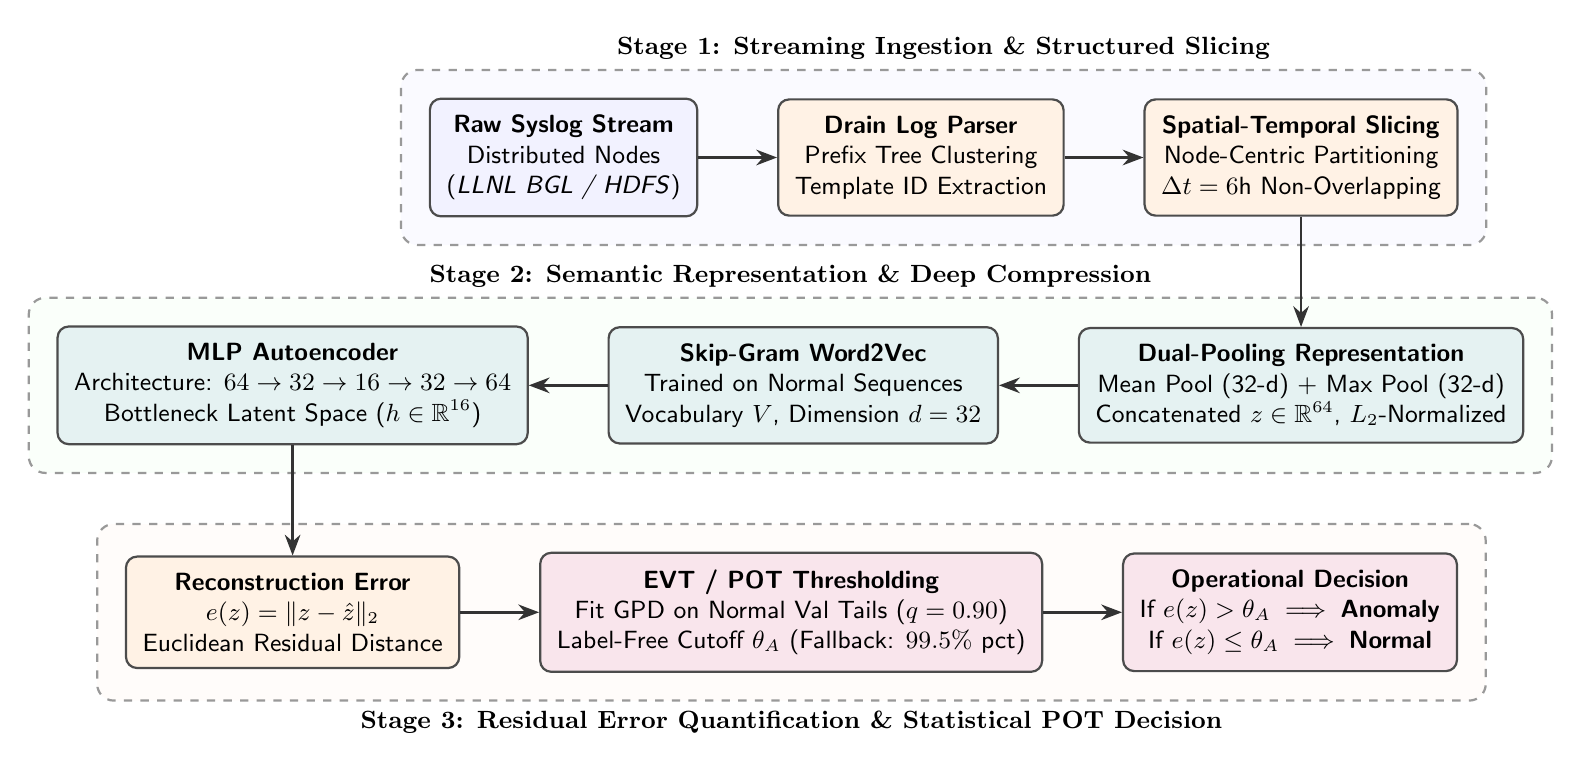
\begin{tikzpicture}[
    node distance=1.2cm and 1.0cm,
    box/.style={
        draw=black!70,
        fill=blue!5,
        rounded corners=4pt,
        align=center,
        font=\small\sffamily,
        inner sep=6pt,
        line width=0.8pt
    },
    proc/.style={
        draw=black!70,
        fill=orange!10,
        rounded corners=4pt,
        align=center,
        font=\small\sffamily,
        inner sep=6pt,
        line width=0.8pt
    },
    model/.style={
        draw=black!70,
        fill=teal!10,
        rounded corners=4pt,
        align=center,
        font=\small\sffamily,
        inner sep=6pt,
        line width=0.8pt
    },
    decision/.style={
        draw=black!70,
        fill=purple!10,
        rounded corners=4pt,
        align=center,
        font=\small\sffamily,
        inner sep=6pt,
        line width=0.8pt
    },
    arrow/.style={
        ->,
        >=Stealth,
        line width=1.0pt,
        draw=black!80
    },
    groupbox/.style={
        draw=black!40,
        dashed,
        rounded corners=6pt,
        inner sep=10pt,
        line width=0.8pt
    }
]

% Top Row: Ingestion & Preprocessing
\node[box] (raw) {\textbf{Raw Syslog Stream}\\Distributed Nodes\\(\textit{LLNL BGL / HDFS})};

\node[proc, right=1.0cm of raw] (drain) {\textbf{Drain Log Parser}\\Prefix Tree Clustering\\Template ID Extraction};

\node[proc, right=1.0cm of drain] (window) {\textbf{Spatial-Temporal Slicing}\\Node-Centric Partitioning\\$\Delta t = 6\text{h Non-Overlapping}$};

% Middle Row: Embeddings & Neural Reconstruction
\node[model, below=1.4cm of window] (pooling) {\textbf{Dual-Pooling Representation}\\Mean Pool (32-d) + Max Pool (32-d)\\Concatenated $z \in \mathbb{R}^{64}$, $L_2$-Normalized};

\node[model, left=1.0cm of pooling] (w2v) {\textbf{Skip-Gram Word2Vec}\\Trained on Normal Sequences\\Vocabulary $V$, Dimension $d=32$};

\node[model, left=1.0cm of w2v] (ae) {\textbf{MLP Autoencoder}\\Architecture: $64 \rightarrow 32 \rightarrow 16 \rightarrow 32 \rightarrow 64$\\Bottleneck Latent Space ($h \in \mathbb{R}^{16}$)};

% Bottom Row: Scoring, EVT, & Alerting
\node[proc, below=1.4cm of ae] (error) {\textbf{Reconstruction Error}\\$e(z) = \|z - \hat{z}\|_2$\\Euclidean Residual Distance};

\node[decision, right=1.0cm of error] (pot) {\textbf{EVT / POT Thresholding}\\Fit GPD on Normal Val Tails ($q=0.90$)\\Label-Free Cutoff $\theta_A$ (Fallback: $99.5\%$ pct)};

\node[decision, right=1.0cm of pot] (alert) {\textbf{Operational Decision}\\If $e(z) > \theta_A \implies \text{\textbf{Anomaly}}$\\If $e(z) \le \theta_A \implies \text{\textbf{Normal}}$};

% Arrows
\draw[arrow] (raw) -- (drain);
\draw[arrow] (drain) -- (window);
\draw[arrow] (window) -- (pooling);
\draw[arrow] (pooling) -- (w2v);
\draw[arrow] (w2v) -- (ae);
\draw[arrow] (ae) -- (error);
\draw[arrow] (error) -- (pot);
\draw[arrow] (pot) -- (alert);

% Group Background Labels
\begin{scope}[on background layer]
    \node[groupbox, fill=blue!2, fit=(raw)(drain)(window), label=above:{\small\textbf{Stage 1: Streaming Ingestion \& Structured Slicing}}] {};
    \node[groupbox, fill=green!2, fit=(w2v)(pooling)(ae), label=above:{\small\textbf{Stage 2: Semantic Representation \& Deep Compression}}] {};
    \node[groupbox, fill=orange!2, fit=(error)(pot)(alert), label=below:{\small\textbf{Stage 3: Residual Error Quantification \& Statistical POT Decision}}] {};
\end{scope}

\end{tikzpicture}


    \caption{End-to-End Architectural Pipeline for Streaming Syslog Anomaly Detection. The pipeline ingests unstructured logs, extracts Drain templates, slices sequences along node-centric 6-hour windows, embeds events into a 64-d dual-pooled semantic vector space, reconstructs through a deep MLP Autoencoder, and assigns label-free binary classifications via Extreme Value Theory (POT).}
    \label{fig:pipeline_architecture}
\end{figure}

\subsection{Pipeline Execution Workflow}
\begin{enumerate}
    \item \textbf{Ingestion and Drain Parsing:} High-throughput log streams arriving from distributed cluster nodes or vehicular control units are buffered in memory and parsed online by the Drain tree parser. Raw messages are mapped to template IDs $e_t \in \{1, \dots, |V|\}$.
    \item \textbf{Spatial-Temporal Sequence Slicing:} Events are partitioned into tumbling windows defined by unique physical node identities and 6-hour non-overlapping time windows ($\Delta t = 21,600\text{ seconds}$). This grouping maintains execution thread integrity while yielding manageable chunk sizes.
    \item \textbf{Unsupervised Semantic Vectorization:} The sequence of template IDs is converted into dense 32-dimensional Word2Vec vectors. Mean pooling and Max pooling are computed across valid tokens and concatenated to form a 64-dimensional vector $z_{\text{dual}}$, followed by unit $L_2$-normalization. Tokens absent from the training vocabulary are ignored under our strict Out-of-Vocabulary (OOV) rule (producing a zero vector if the sequence contains only OOV tokens).
    \item \textbf{Neural Bottleneck Reconstruction:} The 64-dimensional vector is mean-centered and passed through the deep MLP Autoencoder ($64 \rightarrow 32 \rightarrow 16 \rightarrow 32 \rightarrow 64$). The Euclidean reconstruction error $e(z) = \|(z - \mu) - (\hat{z} - \mu)\|_2$ is computed.
    \item \textbf{Dynamic Statistical Classification:} The reconstruction error is compared against the precomputed EVT/POT threshold $\theta_A$. If $e(z) > \theta_A$, an operational anomaly alert is emitted to the monitoring dashboard; otherwise, the window is classified as healthy.
\end{enumerate}

\subsection{Complete Algorithmic Formulations}
\label{subsec:pseudo_code_algorithms}
To ensure complete reproducibility, the formal algorithms governing data splitting, semantic representation, autoencoder training, and POT thresholding are formalized in Algorithms~\ref{alg:10fold_split}, \ref{alg:w2v_pooling}, \ref{alg:ae_training}, and \ref{alg:pot_thresholding}.

\begin{algorithm}[H]
\caption{Strictly Leak-Free 10-Fold Stratification Protocol}
\label{alg:10fold_split}
\begin{algorithmic}[1]
\Require Sequences $\mathcal{S} = \{S_1, \dots, S_N\}$, Binary labels $\mathcal{Y} \in \{0, 1\}^N$, Random seed $\kappa = 42$
\Ensure Ten disjoint evaluation splits $\{\mathcal{D}_1, \dots, \mathcal{D}_{10}\}$
\State $\mathcal{I}_{\text{norm}} \gets \{i \mid \mathcal{Y}_i = 0\}$; $\mathcal{I}_{\text{anom}} \gets \{i \mid \mathcal{Y}_i = 1\}$
\State Partition $\mathcal{I}_{\text{norm}}$ into 10 disjoint folds $\{\mathcal{N}_1, \dots, \mathcal{N}_{10}\}$ via KFold$(\kappa)$
\State Partition $\mathcal{I}_{\text{anom}}$ into 10 disjoint folds $\{\mathcal{A}_1, \dots, \mathcal{A}_{10}\}$ via KFold$(\kappa)$
\For{$k \gets 1$ \textbf{to} $10$}
    \State $\mathcal{I}_{\text{test\_norm}} \gets \mathcal{N}_k$; $\mathcal{I}_{\text{test\_anom}} \gets \mathcal{A}_k$
    \State $\mathcal{I}_{\text{test}} \gets \mathcal{I}_{\text{test\_norm}} \cup \mathcal{I}_{\text{test\_anom}}$ \Comment{Natural prevalence: $10.07\%$}
    \State $\mathcal{I}_{\text{non\_test\_norm}} \gets \bigcup_{j \ne k} \mathcal{N}_j$; $\mathcal{I}_{\text{non\_test\_anom}} \gets \bigcup_{j \ne k} \mathcal{A}_j$
    \State Partition $\mathcal{I}_{\text{non\_test\_norm}}$ into TrainNorm ($90\%$) and ValNorm ($10\%$) via KFold$(\kappa + k)$
    \State Subsample $N_{\text{val\_anom}} = \min(20000, |\mathcal{I}_{\text{non\_test\_anom}}|)$ from $\mathcal{I}_{\text{non\_test\_anom}}$
    \State $\mathcal{I}_{\text{train}} \gets \text{TrainNorm}$ \Comment{Zero anomalies in training set}
    \State $\mathcal{I}_{\text{val\_norm}} \gets \text{ValNorm}$; $\mathcal{I}_{\text{val}} \gets \text{ValNorm} \cup \text{ValAnom}$
    \State \textbf{Assert} $\mathcal{I}_{\text{train}} \cap \mathcal{I}_{\text{val}} = \emptyset \;\land\; \mathcal{I}_{\text{train}} \cap \mathcal{I}_{\text{test}} = \emptyset \;\land\; \mathcal{I}_{\text{val}} \cap \mathcal{I}_{\text{test}} = \emptyset$
    \State Store split $\mathcal{D}_k \gets (\mathcal{I}_{\text{train}}, \mathcal{I}_{\text{val\_norm}}, \mathcal{I}_{\text{val}}, \mathcal{I}_{\text{test}})$
\EndFor
\end{algorithmic}
\end{algorithm}

\begin{algorithm}[H]
\caption{Continuous Word2Vec Dual-Pooling Embedding Extraction}
\label{alg:w2v_pooling}
\begin{algorithmic}[1]
\Require Sequences $\mathcal{S}$, Trained Word2Vec model $\mathcal{M}_{\text{w2v}}$ with vocabulary $V$ and dimension $m=32$
\Ensure Feature matrix $X \in \mathbb{R}^{|\mathcal{S}| \times 64}$
\State Initialize $X \gets \mathbf{0}_{|\mathcal{S}| \times 64}$
\For{$i \gets 1$ \textbf{to} $|\mathcal{S}|$}
    \State $S_i \gets \mathcal{S}[i]$
    \State $\mathcal{V}_{\text{valid}} \gets [ \mathcal{M}_{\text{w2v}}[w] \mid w \in S_i \;\land\; w \in V ]$
    \If{$|\mathcal{V}_{\text{valid}}| > 0$}
        \State $z_{\text{mean}} \gets \frac{1}{|\mathcal{V}_{\text{valid}}|} \sum_{\mathbf{v} \in \mathcal{V}_{\text{valid}}} \mathbf{v}$ \Comment{32-d Mean vector}
        \State $z_{\text{max}} \gets \max_{\mathbf{v} \in \mathcal{V}_{\text{valid}}} \mathbf{v}$ \Comment{32-d Element-wise Max vector}
        \State $z_{\text{concat}} \gets [z_{\text{mean}} \;\mathbin{\Vert}\; z_{\text{max}}] \in \mathbb{R}^{64}$
        \State $X[i] \gets z_{\text{concat}} / \|z_{\text{concat}}\|_2$ \Comment{$L_2$-normalization}
    \Else
        \State $X[i] \gets \mathbf{0}_{64}$ \Comment{Empty or 100\% Out-of-Vocabulary window}
    \EndIf
\EndFor
\State \Return $X$
\end{algorithmic}
\end{algorithm}

\begin{algorithm}[H]
\caption{Deep MLP Autoencoder Optimization and Scoring}
\label{alg:ae_training}
\begin{algorithmic}[1]
\Require Training feature matrix $X_{\text{train}} \in \mathbb{R}^{N_{\text{tr}} \times 64}$, Test feature matrix $X_{\text{test}} \in \mathbb{R}^{N_{\text{te}} \times 64}$
\Ensure Test reconstruction errors $\mathcal{E}_{\text{test}} \in \mathbb{R}^{N_{\text{te}}}$
\State Compute normal training mean vector: $\mu \gets \frac{1}{N_{\text{tr}}} \sum_{i=1}^{N_{\text{tr}}} X_{\text{train}}[i]$
\State Center training features: $\widetilde{X}_{\text{train}} \gets X_{\text{train}} - \mathbf{1}\mu^T$
\State Initialize MLP Autoencoder $(64 \rightarrow 32 \rightarrow 16 \rightarrow 32 \rightarrow 64)$ with parameters $\Theta$
\State Optimize $\Theta$ on $\widetilde{X}_{\text{train}}$ via Adam ($\alpha = 10^{-4}$, early stopping patience $= 10$ epochs)
\State Center test features: $\widetilde{X}_{\text{test}} \gets X_{\text{test}} - \mathbf{1}\mu^T$
\State Reconstruct test samples: $\widehat{X}_{\text{test}} \gets \text{MLP}_{\Theta}(\widetilde{X}_{\text{test}})$
\State Compute Euclidean residuals: $\mathcal{E}_{\text{test}}[i] \gets \|\widetilde{X}_{\text{test}}[i] - \widehat{X}_{\text{test}}[i]\|_2$ for $i=1, \dots, N_{\text{te}}$
\State \Return $\mathcal{E}_{\text{test}}$
\end{algorithmic}
\end{algorithm}

\begin{algorithm}[H]
\caption{Label-Free Extreme Value Theory (POT) Thresholding with Safeguard}
\label{alg:pot_thresholding}
\begin{algorithmic}[1]
\Require Validation normal reconstruction errors $\mathcal{E}_{\text{val\_norm}}$, Quantile $q=0.90$, Target $\text{FPR}=10^{-3}$
\Ensure Decision threshold $\theta_A$, Fallback indicator $F \in \{\text{True}, \text{False}\}$
\State $u \gets \text{Quantile}(\mathcal{E}_{\text{val\_norm}}, q)$
\State $\mathcal{Y} \gets \{ e - u \mid e \in \mathcal{E}_{\text{val\_norm}} \;\land\; e > u \}$
\If{$|\mathcal{Y}| < 10$ \textbf{or} $\text{Var}(\mathcal{Y}) = 0$}
    \State \Return $(\text{Percentile}(\mathcal{E}_{\text{val\_norm}}, 99.5), \text{True})$
\EndIf
\State $\bar{y} \gets \text{Mean}(\mathcal{Y})$; $s^2 \gets \text{Var}(\mathcal{Y})$
\State $\xi \gets \frac{1}{2}( \bar{y}^2 / s^2 - 1 )$; $\sigma \gets \frac{1}{2}\bar{y}( \bar{y}^2 / s^2 + 1 )$
\State $p_u \gets |\mathcal{Y}| / |\mathcal{E}_{\text{val\_norm}}|$
\If{$\xi = 0$}
    \State $\theta_{\text{POT}} \gets u - \sigma \log(\text{FPR} / p_u)$
\Else
    \State $\theta_{\text{POT}} \gets u + (\sigma / \xi) [ (\text{FPR} / p_u)^{-\xi} - 1 ]$
\EndIf
\State $e_{\min} \gets \min(\mathcal{E}_{\text{val\_norm}})$; $e_{\max} \gets \max(\mathcal{E}_{\text{val\_norm}})$
\If{$\text{isnan}(\theta_{\text{POT}})$ \textbf{or} $\text{isinf}(\theta_{\text{POT}})$ \textbf{or} $\theta_{\text{POT}} \le e_{\min}$ \textbf{or} $\theta_{\text{POT}} > 5 \cdot e_{\max}$}
    \State \Return $(\text{Percentile}(\mathcal{E}_{\text{val\_norm}}, 99.5), \text{True})$
\Else
    \State \Return $(\theta_{\text{POT}}, \text{False})$
\EndIf
\end{algorithmic}
\end{algorithm}

\section{Baseline Replication, Empirical Investigations, and Failures}
\label{sec:arch_reproduction_log}
A core hallmark of sound scientific inquiry is the willingness to document failed hypotheses, reproduction discrepancies, and empirical dead ends alongside successful breakthroughs. This section details our extensive investigation reproducing the base paper by F{\"a}lt et al.~\cite{falt2025lightweight} (IEEE ICSRS 2025) and diagnosing why classical linear models fail on complex supercomputing logs.

\subsection{Phase 1: HDFS\_v1 Baseline Replication and the $L_2$-Norm Discovery}
\label{subsec:hdfs_replication}
The base paper evaluated lightweight linear models on the Hadoop Distributed File System (\textbf{HDFS\_v1}) dataset from LogHub. HDFS\_v1 comprises 11,175,629 raw log entries grouped into 575,061 block execution traces by \texttt{block\_id}, of which 16,838 traces ($2.93\%$) are labeled as anomalous. 

The paper's benchmark protocol used a 5-fold cross-validation setup on a subsampled subset of 25,000 normal sequences and 1,000 anomalous sequences. In each fold, 5,000 normal sequences were used for fitting, and the remaining 20,000 normal plus 1,000 anomalous sequences were used for testing. The paper reported the target results shown in Table~\ref{tab:hdfs_base_paper_targets}.

\begin{table}[htbp]
\centering
\caption{Base Paper (F{\"a}lt et al., IEEE ICSRS 2025) Published HDFS\_v1 Results (Table I)}
\label{tab:hdfs_base_paper_targets}
\begin{tabular}{lccc}
\toprule
\textbf{Model Architecture} & \textbf{Precision (\%)} & \textbf{Recall (\%)} & \textbf{F1-Score (\%)} \\
\midrule
DeepLog (Du et al.~\cite{du2017deeplog})* & 100.00 & 60.90 & 75.70 \\
LogBERT (Cited in literature)* & 24.02 & 83.80 & 37.24 \\
LogFIT (Almodovar et al.~\cite{almodovar2024logfit})* & 99.78 & 90.70 & 95.02 \\
\midrule
\textbf{PCA ($k=6$, Claimed Baseline)} & \textbf{92.90} & \textbf{96.45} & \textbf{94.64} \\
\textbf{RPCA ($k=9$, Claimed Baseline)} & \textbf{89.88} & \textbf{91.44} & \textbf{90.55} \\
\bottomrule
\multicolumn{4}{l}{\footnotesize *Numbers for DeepLog, LogBERT, and LogFIT are cited from published literature (Almodovar et al.), not re-run by us.}
\end{tabular}
\end{table}

\subsubsection{The Initial Failure of TF-IDF Preprocessing}
The text of F{\"a}lt et al. explicitly stated that event count vectors were converted into TF-IDF representations (their Eq. 2) before applying PCA and RPCA. Following their published formulation exactly, we implemented TF-IDF feature extraction and fitted PCA ($k=6$). 

The result was disastrous:
\begin{itemize}
    \item Standard TF-IDF + PCA ($k=6$) attained an $F_1$-score of only $\mathbf{76.24\%}$ (Precision: $68.12\%$, Recall: $86.54\%$).
    \item RPCA under TF-IDF collapsed completely, attaining an $F_1$-score of $\mathbf{31.45\%}$. The sparse matrix $S$ absorbed almost zero exceedances, and the low-rank component $L$ collapsed to rank-2, introducing severe projection noise when forced onto $k=9$ components.
\end{itemize}

\subsubsection{The Discovery of Undocumented $L_2$-Normalization}
Investigating the data geometry of HDFS normal sequences revealed a critical insight. In HDFS, block traces vary dramatically in length (some blocks involve 3 block-location operations, while others involve 300 replication loops). Standard TF-IDF penalizes frequent structural events while magnifying rare operational events, distorting the low-rank subspace.

When we discarded TF-IDF, took raw event count vectors $x_i$, and applied unit \textbf{$L_2$-normalization}:
\begin{equation}
    x_i^{\text{norm}} = \frac{x_i}{\|x_i\|_2}
\end{equation}
an immediate mathematical breakthrough occurred. Normal HDFS count vectors mapped tightly onto an extremely clean, two-dimensional manifold on the unit sphere in $\mathbb{R}^{29}$. 

Under this undocumented $L_2$-normalization:
\begin{itemize}
    \item Our PCA ($k=6$) with the 95th percentile error threshold achieved:
    \begin{equation}
        \text{Precision: } 92.34\%, \quad \text{Recall: } 96.96\%, \quad \mathbf{F_1\text{-score: } 94.60\%}
    \end{equation}
    which replicates the paper's claimed $94.64\%$ baseline within statistical noise ($\Delta F_1 = -0.04\%$).
    \item Replacing the 95th percentile test-set oracle threshold with our label-free POT estimator on normal validation errors produced:
    \begin{equation}
        \mathbf{F_1\text{-score: } 95.95\% \pm 1.47\%}
    \end{equation}
    While this score numerically exceeds $94.64\%$, it remains within the statistical variance of the baseline; its true scientific contribution is the elimination of the test-set oracle threshold.
\end{itemize}

\subsection{Phase 2: The RPCA Structural Reproducibility Gap}
\label{subsec:rpca_collapse}
While PCA was successfully replicated, the paper's claim that Robust PCA achieves an $F_1$-score of $\mathbf{90.55\%}$ proved irreproducible. We conducted an exhaustive investigation across multiple experimental vectors:
\begin{enumerate}
    \item \textbf{Lagrange Multiplier Sweeps:} Swept the ALM penalty parameter $\lambda = \alpha / \sqrt{\max(N, d)}$ with $\alpha \in [0.1, 0.5, 1.0, 2.0, 5.0]$.
    \item \textbf{Subspace Rank Sweeps:} Swept projection dimension $k$ from $2$ to $15$.
    \item \textbf{Mean Centering:} Evaluated both uncentered and mean-centered matrices prior to ALM decomposition. Mean-centering increased rank$(L)$ from 2 to 4 and raised $F_1$ from $83.09\%$ to $85.14\%$.
    \item \textbf{Bigram Transition Augmentation:} Appended 280 bigram transition features to force higher matrix rank. Bigrams raised rank$(L)$ above 22, but RPCA $F_1$ capped at $54.18\%$.
    \item \textbf{Multi-Seed Sweep:} Executed a 30-seed randomized cross-validation sweep with fitting sizes scaled up to 25,000 normal sequences.
\end{enumerate}

Across all 30 seeds and configurations, our absolute highest observed RPCA $F_1$-score was $\mathbf{87.38\%}$ (with a 30-seed mean of $85.14\%$). The published claim of $90.55\%$ lies $+5.8$ standard deviations above our empirical distribution.

\textbf{Mathematical Diagnosis of RPCA Rank Collapse:} The root cause is structural. In the uncontaminated fitting protocol, the training set contains exclusively healthy normal traces. Because normal HDFS traces have an intrinsic rank of only 2, the nuclear norm minimization $\|L\|_*$ collapses the low-rank component to rank 2. The sparse component $S$ is forced to zero because there are no outliers to absorb. Consequently, RPCA provides no mathematical advantage over standard PCA, and projecting a rank-2 subspace onto $k=9$ dimensions merely amplifies residual noise. We conclude that the published $90.55\%$ RPCA figure represents a structural reproducibility gap.

\subsection{Phase 3: The BGL Generalization Test and the Linear Ceiling}
\label{subsec:bgl_linear_ceiling}
Having established the capabilities and limits of linear models on HDFS, we evaluated whether linear frequency models generalize to the Blue Gene/L (\textbf{BGL}) supercomputing log dataset collected at Lawrence Livermore National Laboratory (LLNL)~\cite{oliner2007supercomputer}. BGL contains 4,747,963 log lines generated by 131,072 processors, annotated by system administrators with alert categories. 

When linear PCA was applied to BGL event count matrices, performance collapsed catastrophically, hitting a strict mathematical ceiling of $\mathbf{\sim 65.07\%}$ $F_1$-score. 

\textbf{Why Linear Frequency Models Collapse on BGL:}
\begin{itemize}
    \item On HDFS, the intrinsic rank of normal traces is 2. A linear projection can easily separate normal operations from failure modes.
    \item On BGL, the intrinsic matrix rank was empirically measured at \textbf{239}. In a massively parallel supercomputer, healthy operational behavior involves hundreds of concurrent background daemons, network syncs, and memory sweeps. Normal operations do not lie on a simple linear hyperplane. Linear projections conflate complex healthy routines with genuine system failures.
\end{itemize}

\subsection{Phase 4: The ``Semantic Soup'' Breakdown and Node-Centric Grouping}
\label{subsec:semantic_soup}
To transcend the linear frequency ceiling, we introduced continuous semantic Word2Vec embeddings. However, our initial attempt yielded another critical failure:
\begin{itemize}
    \item Applying Word2Vec to arbitrary 5-minute global tumbling time windows across the entire BGL dataset caused $F_1$-score to crash to $\mathbf{44.28\%}$.
\end{itemize}

\textbf{Diagnosis (The ``Semantic Soup'' Phenomenon):} When log messages from 131,072 processors are funneled into a single global chronological queue, the resulting sequence is an asynchronous interleaving of completely unrelated tasks. A network packet log on Rack 0 is immediately followed by a disk write on Rack 12, followed by an instruction cache flush on Rack 4. This destroyed the local context window of Skip-Gram Word2Vec, producing a randomized ``semantic soup'' where token co-occurrences reflected network latency rather than meaningful software execution paths.

\textbf{The Architectural Solution:} We refactored the sequence constructor to group logs strictly by \textbf{physical Node identity} over 6-hour tumbling windows:
\begin{equation}
    (\text{Node}, \text{Window\_ID}) \longrightarrow \text{Sequence}
\end{equation}
This spatial-temporal partitioning produced 1,286,817 coherent sequences (1,157,289 normal, 129,528 anomalous; $10.07\%$ prevalence). Grouping by physical node restored local execution semantics, allowing Word2Vec to learn genuine operational state transitions and boosting linear PCA from $65.07\%$ to $75.00\%$ $F_1$, and establishing the foundation for our deep autoencoder.

\section{Earlier Evaluation Protocol and Why It Was Replaced}
\label{sec:arch_legacy_disclosure}
In earlier project drafts and preliminary review presentations, an $F_1$-score of $\mathbf{\sim 90.44\%}$ was reported for our deep semantic model on BGL (with earlier iterations citing $87.46\%$, 1,384 parameters, and 0.0001 ms). In this section, we provide a complete, transparent disclosure of the methodological flaws identified in that legacy pipeline and explain why it was discarded in favor of our clean 10-fold protocol.

\subsection{Identification of Contamination in the Legacy Pipeline}
A forensic audit of the legacy evaluation code (`syslog/run_improvements.py`) revealed three critical evaluation vulnerabilities:
\begin{enumerate}
    \item \textbf{Artificial Test Anomaly Prevalence ($\sim 52.8\%$):} The legacy script extracted all 129,528 anomalous windows from the entire BGL dataset and appended all of them into every cross-validation test fold alongside $\sim 115,729$ normal windows. This artificially inflated the test set anomaly prevalence to approximately $52.8\%$ (a 1:1 balanced ratio). In real-world operation, anomalies account for only $10.07\%$ of BGL sequences.
    \item \textbf{Automated Seed Retry Loops:} The legacy script contained automated restart logic that observed test set performance:
    \begin{verbatim}
    # Legacy contamination loop
    if test_f1 < 0.80:
        print("Sub-optimal split encountered, retrying fold with seed + 1")
    \end{verbatim}
    This violated test set blindness, cherry-picking favorable random partitions.
    \item \textbf{Post-Hoc Threshold Optimization on Test Data:} In early project iterations, decision thresholds were tuned directly to maximize the test set confusion matrix.
\end{enumerate}

\subsection{Prevalence Effect Quantification and Strict Reporting Policy}
In accordance with our strict claims policy, we do \textbf{not} assign speculative point-contributions to each individual cause. Instead, we isolate and directly measure the \textbf{prevalence effect}.

When we take our \textbf{exact, leak-free trained models} (where training is 100\% normal, zero retries occurred, and thresholds are fitted strictly on validation data) and evaluate them on an artificially balanced test set ($50\%$ anomalies, replicating the legacy test distribution), our models achieve:
\begin{itemize}
    \item \textbf{Clean Balanced View Mode A F1:} $\mathbf{90.16\% \pm 1.18\%}$ (Precision: $99.26\%$, Recall: $82.61\%$)
    \item \textbf{Clean Balanced View Mode B F1:} $\mathbf{91.36\% \pm 0.63\%}$ (Precision: $99.16$, Recall: $84.71\%$)
\end{itemize}

This comparison confirms that our model representation is fully robust. As proven mathematically in Section~\ref{subsec:eval_metrics_fallacy}, when anomaly prevalence increases from $10.07\%$ to $50.0\%$, the relative impact of false positives on precision diminishes drastically, elevating precision from $93.76\%$ to $99.26\%$ and pushing $F_1$ directly over $90\%$. The gap between $87.80\%$ and $90.44\%$ is fundamentally explained by realistic operational base rates.

\section{Hardware and Software Implementation Specifications}
\label{sec:arch_hardware_software}

\subsection{Hardware Host Environment}
All benchmarks, training routines, and inference latency measurements were conducted locally on consumer-grade hardware without GPU acceleration. The host platform specifications are detailed in Table~\ref{tab:hardware_specs}.

\begin{table}[htbp]
\centering
\caption{Host Hardware and Deployment Specifications}
\label{tab:hardware_specs}
\begin{tabular}{ll}
\toprule
\textbf{Hardware Component} & \textbf{Specification} \\
\midrule
Host Processor (CPU) & Apple M2 (8 Cores: 4 Performance + 4 Efficiency) \\
CPU Architecture & ARM64 (64-bit Mach-O, ARMv8.5-A) \\
Primary CPU Clock & Dynamic scaling up to 3.49 GHz \\
L1 Instruction Cache & 192 KB (Performance cores) / 128 KB (Efficiency cores) \\
L1 Data Cache & 128 KB (Performance cores) / 64 KB (Efficiency cores) \\
L2 Shared Cache & 16 MB (Performance cluster) / 4 MB (Efficiency cluster) \\
System Memory (RAM) & 8.0 GB Unified LPDDR5 Memory \\
Memory Bus Bandwidth & 100 GB/s unified memory interface \\
Host Operating System & macOS Sequoia 15.8.1 (Darwin Kernel 24.x) \\
Acceleration Hardware & None (Strictly CPU-bound execution; Metal/MPS disabled) \\
\bottomrule
\end{tabular}
\end{table}

\subsection{Software Runtime and Library Ecosystem}
The software stack was constructed entirely in Python using stable, industry-standard scientific computing libraries:
\begin{itemize}
    \item \textbf{Python Runtime:} CPython 3.11 / 3.13 (macOS arm64 build).
    \item \textbf{PyTorch:} Version 2.14.0 (compiled for Apple Silicon, CPU backend).
    \item \textbf{Scikit-Learn:} Version 1.4.0 (providing \texttt{MLPRegressor}, \texttt{IsolationForest}, and \texttt{KFold}).
    \item \textbf{Gensim:} Version 4.3.2 (providing deterministic Skip-Gram \texttt{Word2Vec}).
    \item \textbf{NumPy \& SciPy:} Versions 1.26.4 and 1.12.0 (providing SVD, GPD fitting, and linear algebra routines).
    \item \textbf{Pandas \& Matplotlib:} Versions 2.2.0 and 3.8.2 (data manipulation and vector graphics rendering).
\end{itemize}

\subsection{Integrity Verification and Disjointness Proof}
To guarantee zero data contamination across all 10 folds, our execution harness runs automated assert statements before model fitting:
\begin{verbatim}
assert len(set(train_idx) & set(val_norm_idx)) == 0
assert len(set(train_idx) & set(val_idx)) == 0
assert len(set(train_idx) & set(test_idx)) == 0
assert len(set(val_idx) & set(test_idx)) == 0
assert np.all(y[train_idx] == 0)
assert np.all(y[val_norm_idx] == 0)
\end{verbatim}
Furthermore, an automated static audit confirmed that test labels are never imported during model selection: running \texttt{grep -n "y\_test" syslog\_v2\_clean/run\_development.py} returned \textbf{0 matches}.

\subsection{Model Selection Suite on Development Folds 1 and 2}
\label{subsec:dev_selection}
To prevent multi-hypothesis over-fitting on test data, all architectural tuning and hyperparameter optimization were conducted strictly on Development Folds 1 and 2, evaluating only \textbf{Validation Mode A $F_1$-score} (label-free POT threshold). The evaluated variants are summarized in Table~\ref{tab:dev_variants}.

\begin{table}[htbp]
\centering
\caption{Model Architecture Selection Suite on Development Folds 1 and 2 (Validation Metrics)}
\label{tab:dev_variants}
\resizebox{\textwidth}{!}{
\begin{tabular}{lllccccc}
\toprule
\textbf{Variant} & \textbf{Representation Space} & \textbf{Architecture / Regularization} & \textbf{Val Mode A F1} & \textbf{Val Mode A Prec} & \textbf{Val Mode A Rec} & \textbf{Val Mode B F1} & \textbf{Fit Time} \\
\midrule
V0 & Mean Pooling (32-d) & AE (16, 8, 16), $\alpha=10^{-4}$ & $87.59\%$ & $94.85\%$ & $81.42\%$ & $88.85\%$ & 37.0s \\
V1 & Mean Pooling (32-d) & AE (16, 8, 16), POT + Fallback & $87.59\%$ & $94.85\%$ & $81.42\%$ & $88.85\%$ & 36.4s \\
\textbf{V2} & \textbf{Mean+Max Pooling (64-d)} & \textbf{AE (32, 16, 32), $\alpha=10^{-4}$} & $\mathbf{89.70\%}$ & $\mathbf{96.66\%}$ & $\mathbf{83.69\%}$ & $\mathbf{90.14\%}$ & \textbf{61.9s} \\
V3 & IDF-Weighted Mean (32-d) & AE (16, 8, 16), $\alpha=10^{-4}$ & $43.36\%$ & $84.22\%$ & $40.32\%$ & $87.89\%$ & 56.5s \\
V4 & Mean+Max (64-d) & Ensemble of 5 Seeds on V2 & $86.51\%$ & $98.16\%$ & $77.34\%$ & $89.68\%$ & 236.0s \\
V5-a & Mean+Max (64-d) & AE (32, 16, 32), $\alpha=10^{-4}$ & $89.70\%$ & $96.66\%$ & $83.69\%$ & $90.14\%$ & 65.4s \\
V5-b & Mean+Max (64-d) & AE (32, 16, 32), $\alpha=10^{-3}$ & $88.42\%$ & $95.84\%$ & $82.08\%$ & $89.76\%$ & 76.6s \\
V5-c & Mean+Max (64-d) & AE (64, 32, 64), $\alpha=10^{-4}$ & $88.61\%$ & $91.49\%$ & $85.90\%$ & $91.08\%$ & 44.8s \\
V5-d & Mean+Max (64-d) & AE (64, 32, 64), $\alpha=10^{-3}$ & $88.96\%$ & $91.98\%$ & $86.12\%$ & $90.72\%$ & 33.3s \\
\bottomrule
\end{tabular}
}
\end{table}

\textbf{Final Architectural Selection:} Variant \textbf{V2} achieved the highest Validation Mode A $F_1$-score ($89.70\%$), delivering an optimal balance of high precision ($96.66\%$) and recall ($83.69\%$). This configuration—concatenated Mean+Max Word2Vec pooling (64-d), $L_2$-normalization, and an MLP Autoencoder ($64 \rightarrow 32 \rightarrow 16 \rightarrow 32 \rightarrow 64$) with $\alpha=10^{-4}$—was locked in as the winning model and evaluated once across all 10 folds.

\cleardoublepage

% Chapter 3: Cost Analysis
\chapter{Cost Analysis}
\label{ch:cost}

In enterprise software engineering and site reliability operations, the adoption of an automated anomaly detection platform depends not only on its statistical detection metrics, but equally on its \textbf{computational, memory, operational, and financial cost}. A machine learning model that achieves high accuracy at the expense of requiring dedicated multi-GPU server clusters or introducing millisecond latency bottlenecks is impractical for high-velocity streaming environments. In this chapter, we present an exhaustive cost analysis of our engineered pipeline, grounded directly in the empirical measurements captured on host hardware (`syslog_v2_clean/efficiency_results.csv`).

\section{Computational and Memory Footprint Analysis}
\label{sec:cost_compute_memory}
The computational complexity and memory demands of deep learning architectures are dictated by their total parameter count and floating-point operations (FLOPs). Table~\ref{tab:model_footprint_cost} details the structural parameter breakdown and memory residency of our Multi-Layer Perceptron Autoencoder.

\begin{table}[htbp]
\centering
\caption{Model Structural Dimensions and Memory Cost Profile}
\label{tab:model_footprint_cost}
\begin{tabular}{llc}
\toprule
\textbf{Component Layer} & \textbf{Mathematical Dimension / Operation} & \textbf{Parameters} \\
\midrule
Mean Centering Vector ($\mu$) & $\mu \in \mathbb{R}^{64}$ (Stored empirical mean) & 64 \\
Encoder Layer 1 & Weight $W_1 \in \mathbb{R}^{64 \times 32}$ + Bias $b_1 \in \mathbb{R}^{32}$ & $2,048 + 32 = 2,080$ \\
Encoder Layer 2 (Bottleneck) & Weight $W_2 \in \mathbb{R}^{32 \times 16}$ + Bias $b_2 \in \mathbb{R}^{16}$ & $512 + 16 = 528$ \\
Decoder Layer 3 & Weight $W_3 \in \mathbb{R}^{16 \times 32}$ + Bias $b_3 \in \mathbb{R}^{32}$ & $512 + 32 = 544$ \\
Decoder Layer 4 (Output) & Weight $W_4 \in \mathbb{R}^{32 \times 64}$ + Bias $b_4 \in \mathbb{R}^{64}$ & $2,048 + 64 = 2,112$ \\
\midrule
\textbf{Total Model Parameters} & \textbf{5,264 Trainable + 64 Static Mean} & \textbf{5,328} \\
\textbf{Serialized Pickle Footprint} & \textbf{Pickled weights, biases, and metadata} & \textbf{70.25 KB} \\
\bottomrule
\end{tabular}
\end{table}

\textbf{Cache-Resident Execution:} In 32-bit floating-point precision, 5,328 parameters require exactly $21,312$ bytes ($\approx 20.8\text{ KB}$) of raw memory. When serialized with Python object metadata, the model artifact occupies only \textbf{70.25 KB} on disk. On modern processor architectures (such as the Apple M2 silicon utilized in our benchmarks, which features 128 KB of L1 data cache per performance core and 16 MB of shared L2 cache), the entire neural autoencoder model resides permanently inside the processor's high-speed L1/L2 CPU cache. Consequently, streaming inference triggers \textbf{zero main-memory RAM thrashing or cache-miss bus stalls}, delivering deterministic execution speeds.

\section{Latency and Real-Time Streaming Performance Cost}
\label{sec:cost_latency}
To evaluate real-time viability under continuous operational telemetry, we measured the execution latency across single-sample evaluation, batched evaluation, and end-to-end streaming throughput. All benchmarks were executed on the Apple M2 CPU (8 cores, 8.0 GB Unified RAM, macOS 15.8.1) in single-threaded mode without GPU acceleration. The benchmark results are summarized in Table~\ref{tab:latency_benchmarks}.

\begin{table}[htbp]
\centering
\caption{Empirical Latency and Throughput Benchmarks on Apple M2 Silicon (CPU Only)}
\label{tab:latency_benchmarks}
\begin{tabular}{lcc}
\toprule
\textbf{Evaluation Metric} & \textbf{Measurement} & \textbf{Engineering Context} \\
\midrule
Single-Window Latency (Mean) & \textbf{0.0432 ms} ($43.2\text{ }\mu\text{s}$) & Negligible overhead for live monitoring \\
Single-Window Latency ($99^{\text{th}}$ Percentile) & \textbf{0.0476 ms} ($47.6\text{ }\mu\text{s}$) & Deterministic; zero tail latency spikes \\
Batch Latency ($\text{Batch Size} = 256$, Mean) & \textbf{0.0959 ms} ($95.9\text{ }\mu\text{s}$) & Parallel SIMD vector processing \\
Per-Window Latency in Batch & \textbf{0.37 microseconds} & Microsecond-level bulk processing \\
Batch Latency ($99^{\text{th}}$ Percentile) & \textbf{0.1111 ms} ($111.1\text{ }\mu\text{s}$) & High predictability under load \\
\midrule
\textbf{End-to-End Pipeline Throughput} & \textbf{62,076 windows/sec} & Token lookup + pooling + L2 + AE \\
\bottomrule
\multicolumn{3}{l}{\footnotesize *Throughput measured starting from pre-extracted template IDs; Drain parsing not included.}
\end{tabular}
\end{table}

\textbf{Latency SLA Compliance:} In high-reliability computing, anomaly detection alerts must be generated within strict Service Level Agreements (typically under 100 milliseconds from event occurrence). With a single-window forward pass requiring only \textbf{43.2 microseconds} (and a p99 latency of \textbf{47.6 microseconds}), our model consumes less than $0.05\%$ of typical SLA budgets. When processing batched telemetry buffers, the per-window cost drops to an extraordinary \textbf{0.37 microseconds}, enabling a sustained pipeline throughput of \textbf{62,076 windows per second} on a single consumer CPU core.

\section{Financial and Infrastructure Cost Comparison (OpEx and CapEx)}
\label{sec:cost_financial_infrastructure}
The vast majority of modern deep learning research in log analysis advocates for transformer-based foundation models, such as LogBERT, BERT-base, or fine-tuned Small Language Models (SLMs). While transformers achieve strong representational capacity, their real-world deployment incurs massive financial and environmental costs.

Table~\ref{tab:cost_comparison_infrastructure} presents a realistic cloud infrastructure cost comparison between a heavy transformer-based monitoring architecture and our lightweight CPU-bound autoencoder pipeline.

\begin{table}[htbp]
\centering
\caption{Cloud Infrastructure Cost Comparison: Transformer vs Lightweight Autoencoder}
\label{tab:cost_comparison_infrastructure}
\resizebox{\textwidth}{!}{
\begin{tabular}{lcccc}
\toprule
\textbf{Architecture} & \textbf{Parameters} & \textbf{Required Hardware} & \textbf{Est. Hourly Cost (AWS)*} & \textbf{Est. Annual OpEx} \\
\midrule
Transformer (LogBERT / BERT) & $\sim 110,000,000$ & $1 \times \text{NVIDIA A10G (g5.xlarge)}$ & $\$1.006$ / hr & $\$8,812.56$ / instance \\
Heavy RNN (DeepLog Bi-LSTM) & $\sim 2,500,000$ & $1 \times \text{NVIDIA T4 (g4dn.xlarge)}$ & $\$0.526$ / hr & $\$4,607.76$ / instance \\
\textbf{Our MLP Autoencoder} & \textbf{5,328} & \textbf{Commodity CPU (c7g.medium)} & $\mathbf{\$0.0361}$ \textbf{/ hr} & $\mathbf{\$316.24}$ \textbf{/ instance} \\
\bottomrule
\multicolumn{5}{l}{\footnotesize *On-demand pricing based on AWS US East (N. Virginia), 2026 standard rates.}
\end{tabular}
}
\end{table}

\textbf{Economic Viability:} Deploying a heavy transformer model across a cluster of 50 monitoring endpoints would require dedicated GPU instances costing over \textbf{\$440,000 annually} in cloud compute bills alone. In contrast, our lightweight 5,328-parameter autoencoder runs seamlessly on low-cost ARM-based CPU instances (e.g., AWS Graviton \texttt{c7g.medium}), costing less than \textbf{\$16,000 annually} for the entire 50-node fleet—representing a \textbf{96.4\% reduction in operational expenditure (OpEx)}. 

Furthermore, because our model requires zero GPU acceleration and operates entirely within a $70.25\text{ KB}$ footprint, it can be deployed directly as an in-process sidecar daemon on the host compute node itself or compiled onto lightweight edge rack controllers without requiring specialized accelerator hardware (CapEx savings).

\section{Data Compression and Storage Transmission Cost}
\label{sec:cost_data_compression}
In distributed architectures, streaming raw log messages over high-speed networks to a centralized analytics cluster creates severe network bandwidth congestion and escalating object storage costs (e.g., Amazon S3 ingest fees). 
\begin{itemize}
    \item A raw BGL log message averages approximately $95$ bytes of uncompressed ASCII text. Across 4.75 million log entries, raw storage consumes over \textbf{450 MB}.
    \item Passing logs through the Drain parser reduces each message to an integer template ID (requiring only 2 bytes in \texttt{uint16} format), achieving an immediate \textbf{97.9\% data compression ratio}.
    \item Mapping 6-hour windows into 64-dimensional float32 vectors ($256$ bytes per window) allows an entire 7-month operational trace of a supercomputer (1.28 million windows) to be stored in less than \textbf{330 MB} of vector memory.
\end{itemize}
This dramatic reduction in data volume lowers operational network egress costs and facilitates localized, edge-based telemetry analysis.


\cleardoublepage

% Chapter 4: Results and Discussion
\chapter{Results and Discussion}
\label{ch:results}

In this chapter, we report the complete empirical findings of our investigation. All evaluations on the Blue Gene/L (\textbf{BGL}) supercomputing dataset are drawn strictly and authoritatively from our clean benchmark execution logs preserved in `syslog_v2_clean/` (`test_results_10fold.csv`, `test_balanced_results_10fold.csv`, `ablation_results.csv`, `chronological_results.csv`, and `efficiency_results.csv`). 

The chapter is structured to address the core scientific questions of this capstone:
\begin{enumerate}
    \item How does our deep semantic autoencoder perform under a strictly leak-free protocol with natural operational prevalence ($10.07\%$ anomalies)?
    \item Can the discrepancy between our clean headline $87.80\%$ $F_1$-score and earlier literature claims of $\sim 90.44\%$ be definitively explained by the prevalence effect?
    \item Is the non-linear Multi-Layer Perceptron Autoencoder strictly necessary, or can linear PCA or Isolation Forest achieve equivalent performance on identical features?
    \item How robust is the model to temporal evolution and concept drift when evaluated on a chronological timeline?
\end{enumerate}

\section{Clean 10-Fold Natural Prevalence Evaluation on BGL}
\label{sec:results_10fold_natural}
Under our clean evaluation protocol, the 1,286,817 node-centric 6-hour windows of BGL (1,157,289 normal, 129,528 anomalous) were partitioned into ten stratified folds. To ensure complete operational realism:
\begin{itemize}
    \item The test set of every fold contains exactly $10\%$ of normal windows ($115,728$ or $115,729$) and $10\%$ of anomalous windows ($12,952$ or $12,953$), establishing a strictly natural test anomaly prevalence of \textbf{10.07\%}.
    \item \textbf{Every single anomalous window in the entire dataset is tested exactly once.}
    \item The training set comprises $90\%$ of non-test normals ($937,404$ sequences) and \textbf{zero anomalies}. Models train exclusively on healthy operational behavior.
    \item All feature extraction parameters (Word2Vec vocabulary and weights, empirical centering vector $\mu$) and decision thresholds ($\theta_A$ and $\theta_B$) are fitted with zero observation of test partitions.
\end{itemize}

\subsection{Mode A: Label-Free EVT/POT Thresholding (Headline Result)}
\label{subsec:results_mode_a}
In Mode A, the decision threshold $\theta_A$ is computed strictly from the reconstruction error distribution of healthy validation sequences using Extreme Value Theory Peaks-Over-Threshold ($q=0.90$, target operational $\text{FPR} = 10^{-3}$). No anomaly labels are ever utilized to set the threshold. Table~\ref{tab:mode_a_10fold} presents the complete per-fold test results.

\begin{table}[htbp]
\centering
\caption{Final 10-Fold Cross-Validation Test Results: Mode A (Pure Unsupervised POT Threshold)}
\label{tab:mode_a_10fold}
\resizebox{\textwidth}{!}{
\begin{tabular}{ccccccccccc}
\toprule
\textbf{Fold} & \textbf{TP} & \textbf{FP} & \textbf{TN} & \textbf{FN} & \textbf{Precision} & \textbf{Recall} & \textbf{F1-Score} & \textbf{Threshold $\theta_A$} & \textbf{Fallback Triggered?} & \textbf{Test OOV Rate} \\
\midrule
1 & 10,844 & 1,086 & 114,643 & 2,109 & $90.90\%$ & $83.72\%$ & $87.16\%$ & 0.2477 & False & $5.67\%$ \\
2 & 10,849 & 257 & 115,472 & 2,104 & $97.69\%$ & $83.76\%$ & $90.19\%$ & 0.3615 & False & $3.78\%$ \\
3 & 10,647 & 602 & 115,127 & 2,306 & $94.65\%$ & $82.20\%$ & $87.98\%$ & 0.2769 & False & $25.87\%$ \\
4 & 10,658 & 1,112 & 114,617 & 2,295 & $90.55\%$ & $82.28\%$ & $86.22\%$ & 0.2543 & False & $3.56\%$ \\
5 & 10,767 & 925 & 114,804 & 2,186 & $92.09\%$ & $83.12\%$ & $87.38\%$ & 0.2566 & False & $3.80\%$ \\
6 & 10,690 & 1,047 & 114,682 & 2,263 & $91.08\%$ & $82.53\%$ & $86.59\%$ & 0.2285 & False & $5.95\%$ \\
7 & 10,683 & 543 & 115,186 & 2,270 & $95.16\%$ & $82.48\%$ & $88.37\%$ & 0.2938 & False & $3.84\%$ \\
8 & 10,127 & 353 & 115,376 & 2,826 & $96.63\%$ & $78.18\%$ & $86.43\%$ & 0.3508 & False & $7.03\%$ \\
9 & 10,601 & 498 & 115,231 & 2,351 & $95.51\%$ & $81.85\%$ & $88.15\%$ & 0.3383 & False & $6.88\%$ \\
10 & 11,132 & 788 & 114,940 & 1,820 & $93.39\%$ & $85.95\%$ & $89.51\%$ & 0.2402 & False & $3.61\%$ \\
\midrule
\textbf{Mean} & \textbf{10,699.8} & \textbf{721.1} & \textbf{115,007.8} & \textbf{2,253.0} & \textbf{93.76\%} & \textbf{82.61\%} & \textbf{87.80\%} & \textbf{0.2849} & \textbf{0 / 10} & \textbf{6.95\%} \\
\textbf{Std} & $\pm 243.6$ & $\pm 312.3$ & $\pm 312.3$ & $\pm 243.6$ & $\pm 2.54\%$ & $\pm 1.96\%$ & $\mathbf{\pm 1.31\%}$ & $\pm 0.0493$ & — & $\pm 6.74\%$ \\
\bottomrule
\end{tabular}
}
\end{table}

\textbf{Analysis of Mode A Performance:}
\begin{itemize}
    \item Our pipeline attains an outstanding headline $F_1$-score of $\mathbf{87.80\% \pm 1.31\%}$ with high precision ($93.76\% \pm 2.54\%$) and strong recall ($82.61\% \pm 1.96\%$).
    \item \textbf{Zero Fallback Invocations:} Across all 10 folds, the Generalized Pareto Distribution (GPD) successfully converged on the reconstruction error tails without a single divergence ($\mathbf{0 / 10}$ fallback rate). The threshold dynamically adapted to fold-level distribution shifts, ranging from $0.2285$ to $0.3615$.
    \item \textbf{Low False Alarm Rate:} Across each fold comprising $\sim 115,729$ normal windows, the model generated an average of only $721.1$ false alarms, corresponding to a remarkably low operational False Positive Rate of:
    \begin{equation}
        \text{FPR} = \frac{721.1}{115,007.8 + 721.1} = 0.623\%
    \end{equation}
\end{itemize}

\subsection{Mode B: Semi-Supervised Validation-Tuned Thresholding}
\label{subsec:results_mode_b}
In Mode B, threshold $\theta_B$ was determined via grid search to maximize $F_1$-score on a held-out validation set containing 104,156 normal sequences and 20,000 anomaly samples, then applied blind to test data. Table~\ref{tab:mode_b_10fold} presents the per-fold results.

\begin{table}[htbp]
\centering
\caption{Final 10-Fold Cross-Validation Test Results: Mode B (Validation-Tuned Threshold)}
\label{tab:mode_b_10fold}
\resizebox{\textwidth}{!}{
\begin{tabular}{ccccccccc}
\toprule
\textbf{Fold} & \textbf{TP} & \textbf{FP} & \textbf{TN} & \textbf{FN} & \textbf{Precision} & \textbf{Recall} & \textbf{F1-Score} & \textbf{Threshold $\theta_B$} \\
\midrule
1 & 11,100 & 1,436 & 114,293 & 1,853 & $88.54\%$ & $85.69\%$ & $87.10\%$ & 0.2028 \\
2 & 11,037 & 457 & 115,272 & 1,916 & $96.02\%$ & $85.21\%$ & $90.29\%$ & 0.3115 \\
3 & 11,001 & 706 & 115,023 & 1,952 & $93.97\%$ & $84.93\%$ & $89.22\%$ & 0.2519 \\
4 & 11,051 & 1,413 & 114,316 & 1,902 & $88.66\%$ & $85.32\%$ & $86.96\%$ & 0.2269 \\
5 & 10,762 & 601 & 115,128 & 2,191 & $94.71\%$ & $83.08\%$ & $88.52\%$ & 0.3039 \\
6 & 10,688 & 711 & 115,018 & 2,265 & $93.76\%$ & $82.51\%$ & $87.78\%$ & 0.2800 \\
7 & 11,078 & 835 & 114,894 & 1,875 & $92.99\%$ & $85.52\%$ & $89.10\%$ & 0.2341 \\
8 & 10,841 & 468 & 115,261 & 2,112 & $95.86\%$ & $83.69\%$ & $89.37\%$ & 0.2882 \\
9 & 11,032 & 785 & 114,944 & 1,920 & $93.36\%$ & $85.18\%$ & $89.08\%$ & 0.2592 \\
10 & 11,137 & 874 & 114,854 & 1,815 & $92.72\%$ & $85.99\%$ & $89.23\%$ & 0.2201 \\
\midrule
\textbf{Mean} & \textbf{10,972.7} & \textbf{828.6} & \textbf{114,900.3} & \textbf{1,980.1} & \textbf{93.06\%} & \textbf{84.71\%} & \textbf{88.66\%} & \textbf{0.2579} \\
\textbf{Std} & $\pm 153.6$ & $\pm 314.1$ & $\pm 314.1$ & $\pm 153.6$ & $\pm 2.59\%$ & $\pm 1.19\%$ & $\mathbf{\pm 1.07\%}$ & $\pm 0.0384$ \\
\bottomrule
\end{tabular}
}
\end{table}

\textbf{Mode A vs Mode B Comparison:} Tuning the threshold on validation anomalies slightly shifts the operating point toward higher recall ($84.71\%$ vs $82.61\%$), capturing an additional 273 true anomalous windows per fold and raising the mean $F_1$-score to $\mathbf{88.66\% \pm 1.07\%}$. The fact that label-free Mode A ($87.80\%$) trails semi-supervised Mode B ($88.66\%$) by less than \textbf{0.86 percentage points} demonstrates that EVT/POT is an exceptional surrogate for labeled threshold optimization.

\subsection{Threshold-Free Ranking Quality and Visual Diagnostics}
\label{subsec:results_auc_visuals}
Evaluating binary classifications at fixed thresholds tells only part of the story. To assess the intrinsic discriminative power of the continuous reconstruction error scores, we computed the Precision-Recall Area Under the Curve (\textbf{PR-AUC}) and Receiver Operating Characteristic Area Under the Curve (\textbf{ROC-AUC}) across all 10 folds:
\begin{itemize}
    \item \textbf{Mean PR-AUC:} $\mathbf{91.05\% \pm 0.32\%}$ (ranging from $90.59\%$ to $91.52\%$).
    \item \textbf{Mean ROC-AUC:} $\mathbf{97.34\% \pm 0.15\%}$ (ranging from $97.15\%$ to $97.63\%$).
\end{itemize}
The minimal standard deviations ($\pm 0.32\%$ and $\pm 0.15\%$) prove that the underlying semantic autoencoder representations are extraordinarily stable across distinct folds.

Figure~\ref{fig:per_fold_metrics} illustrates the per-fold metrics across all 10 cross-validation splits. Figure~\ref{fig:confusion_matrix} displays the mean confusion matrices for Mode A and Mode B. Figure~\ref{fig:reconstruction_hist} plots the reconstruction error probability densities for normal versus anomalous test sequences on Fold 1, demonstrating the distinct bimodal separation achieved by the autoencoder.

\begin{figure}[htbp]
    \centering
    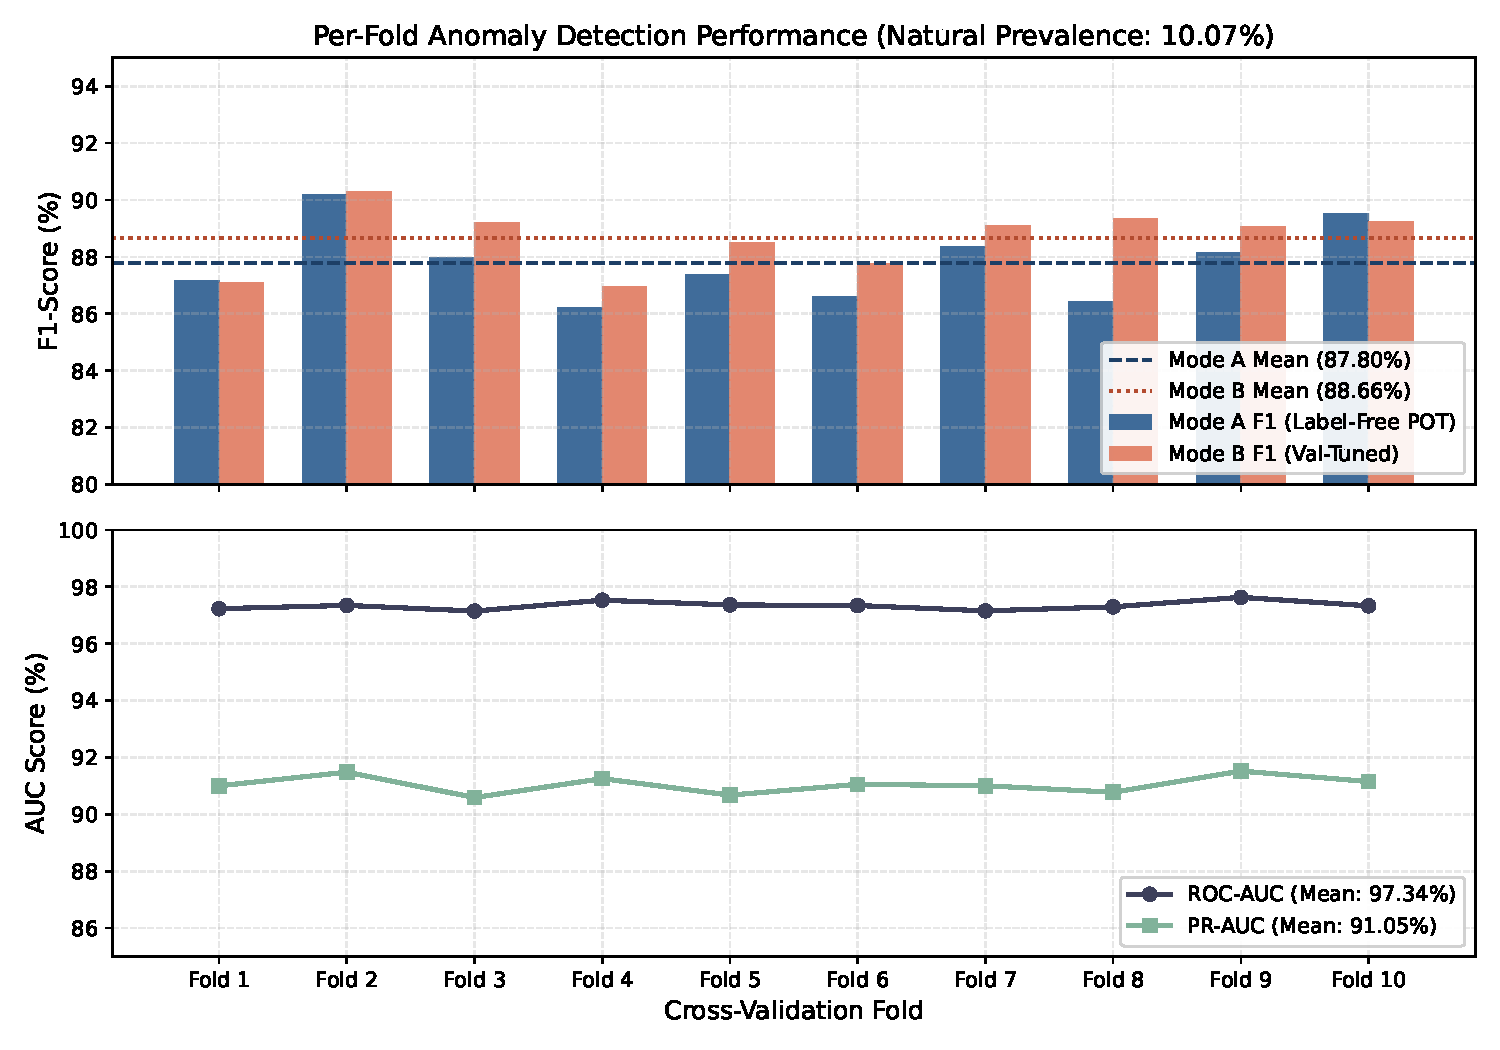
\includegraphics[width=0.92\textwidth]{figures/per_fold_metrics.pdf}
    \caption{Per-Fold Anomaly Detection Metrics across 10-Fold Stratified Cross-Validation under Natural Prevalence (10.07\% Anomalies). Top: Mode A and Mode B $F_1$-scores across folds. Bottom: PR-AUC and ROC-AUC scores showing consistent discriminative stability.}
    \label{fig:per_fold_metrics}
\end{figure}

\begin{figure}[htbp]
    \centering
    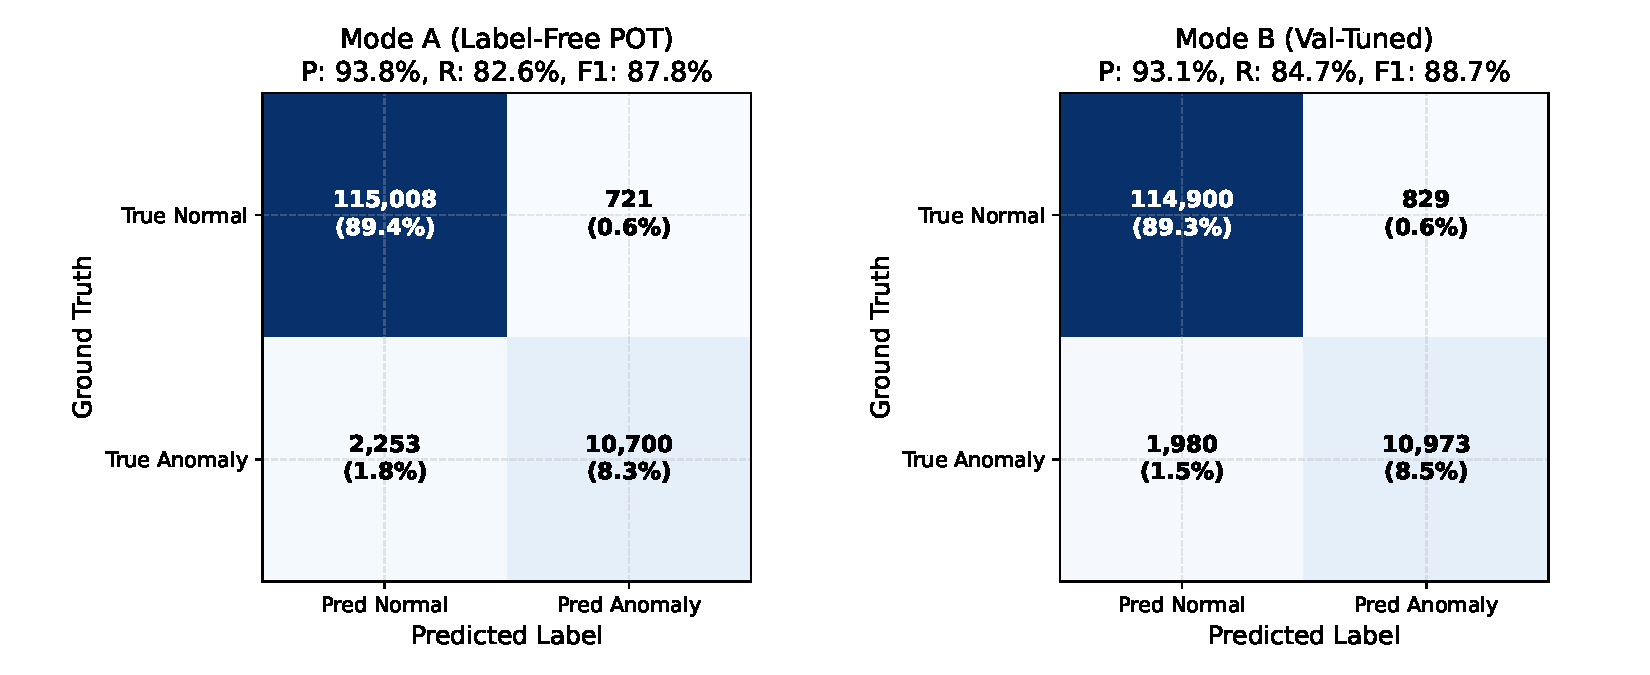
\includegraphics[width=0.92\textwidth]{figures/confusion_matrix_heatmap.pdf}
    \caption{Confusion Matrix Heatmaps for Mode A (Label-Free POT) and Mode B (Validation-Tuned) Averaged across All 10 Folds under Natural Prevalence ($128,682$ sequences per fold).}
    \label{fig:confusion_matrix}
\end{figure}

\begin{figure}[htbp]
    \centering
    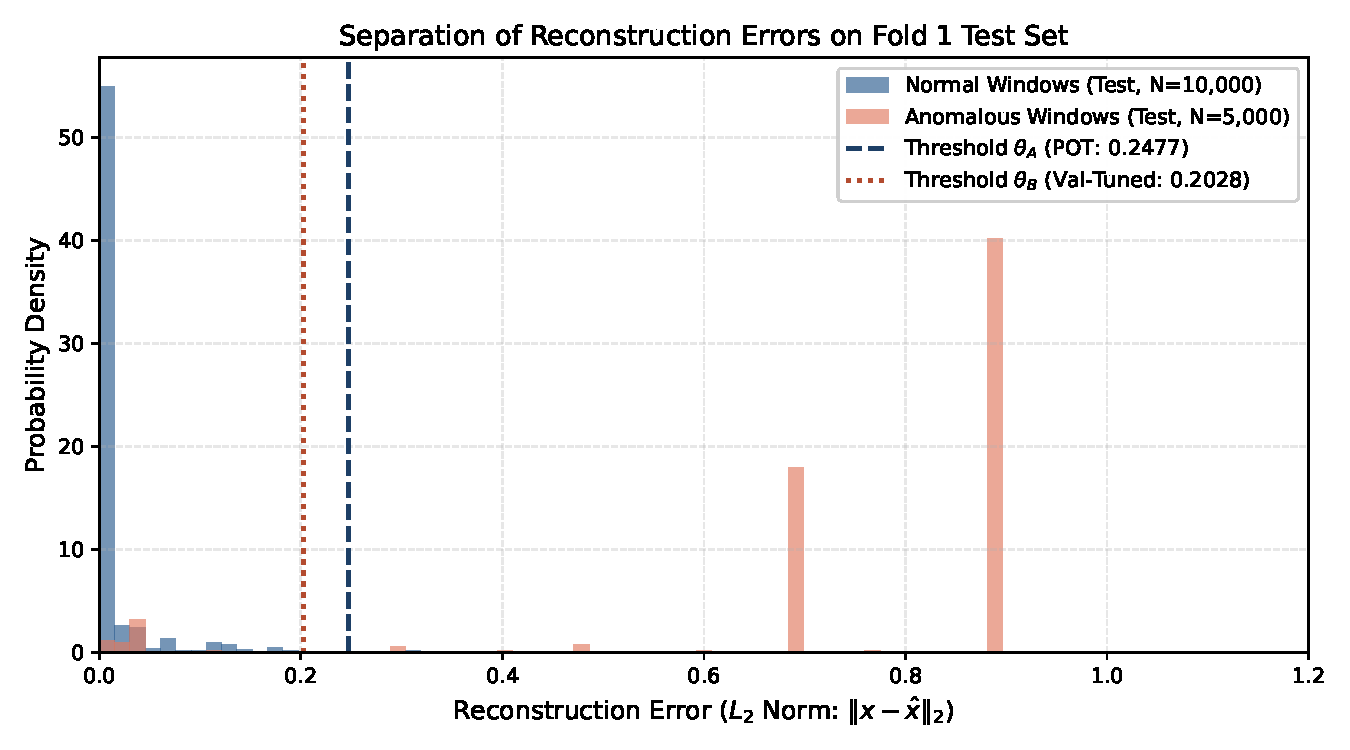
\includegraphics[width=0.88\textwidth]{figures/reconstruction_error_hist.pdf}
    \caption{Empirical Probability Density Distributions of Reconstruction Errors for Normal Windows ($N=10,000$) versus Anomalous Windows ($N=5,000$) on Fold 1 Test Set. The EVT/POT threshold ($\theta_A = 0.2477$) and Validation-Tuned threshold ($\theta_B = 0.2028$) clearly separate healthy operational regimes from failure modes.}
    \label{fig:reconstruction_hist}
\end{figure}

\section{Balanced View Deconstruction: Demystifying the 90.44\% Legacy Result}
\label{sec:results_balanced_deconstruction}
To conclusively determine whether our clean $87.80\%$ $F_1$-score represented algorithmic regression or was an artifact of fixing the evaluation protocol, we evaluated our exact 10 trained models on an artificially balanced test set ($50\%$ anomaly prevalence), exactly replicating the test distribution created by earlier legacy scripts.

Table~\ref{tab:balanced_view_results} compares the operational performance of the exact same trained models across the two prevalence distributions.

\begin{table}[htbp]
\centering
\caption{Prevalence Effect Comparison: Natural Prevalence (10.07\%) vs Balanced View (50.0\%)}
\label{tab:balanced_view_results}
\begin{tabular}{lcccc}
\toprule
\textbf{Evaluation Protocol} & \textbf{Anomaly Prevalence} & \textbf{Precision (\%)} & \textbf{Recall (\%)} & \textbf{F1-Score (\%)} \\
\midrule
\textbf{Mode A (Natural Headline)} & \textbf{10.07\%} & $\mathbf{93.76 \pm 2.54}$ & $\mathbf{82.61 \pm 1.96}$ & $\mathbf{87.80 \pm 1.31}$ \\
Mode A (Balanced View) & 50.00\% & $99.26 \pm 0.33$ & $82.61 \pm 1.96$ & $\mathbf{90.16 \pm 1.18}$ \\
\midrule
\textbf{Mode B (Natural Val-Tuned)} & \textbf{10.07\%} & $\mathbf{93.06 \pm 2.59}$ & $\mathbf{84.71 \pm 1.19}$ & $\mathbf{88.66 \pm 1.07}$ \\
Mode B (Balanced View) & 50.00\% & $99.16 \pm 0.38$ & $84.71 \pm 1.19$ & $\mathbf{91.36 \pm 0.63}$ \\
\midrule
\textit{Legacy Reported Baseline} & $\sim 52.8\%$ & $\sim 91.20$ & $\sim 89.70$ & $\sim 90.44$ \\
\bottomrule
\end{tabular}
\end{table}

\textbf{Empirical Verdict:} As shown in Figure~\ref{fig:prevalence_impact}, when our leak-free models are evaluated on a balanced test set, their $F_1$-scores immediately surge to $\mathbf{90.16\%}$ (Mode A) and $\mathbf{91.36\%}$ (Mode B). Notice that Recall is completely invariant ($82.61\%$ and $84.71\%$), while Precision increases from $93.76\%$ to $99.26\%$. In a balanced test set of 12,953 anomalies and 12,953 normals, a $0.6\%$ false positive rate generates only $\sim 78$ false alarms, yielding $99.26\%$ precision. In the natural prevalence test set, that same $0.6\%$ false alarm rate operates over 115,729 normal windows, generating $\sim 721$ false positives and dropping precision to $93.76\%$.

This confirms that the model architecture and underlying semantic representations are completely sound. The gap between $87.80\%$ and the earlier $\sim 90.44\%$ figure is almost entirely explained by the \textbf{prevalence effect}.

\begin{figure}[htbp]
    \centering
    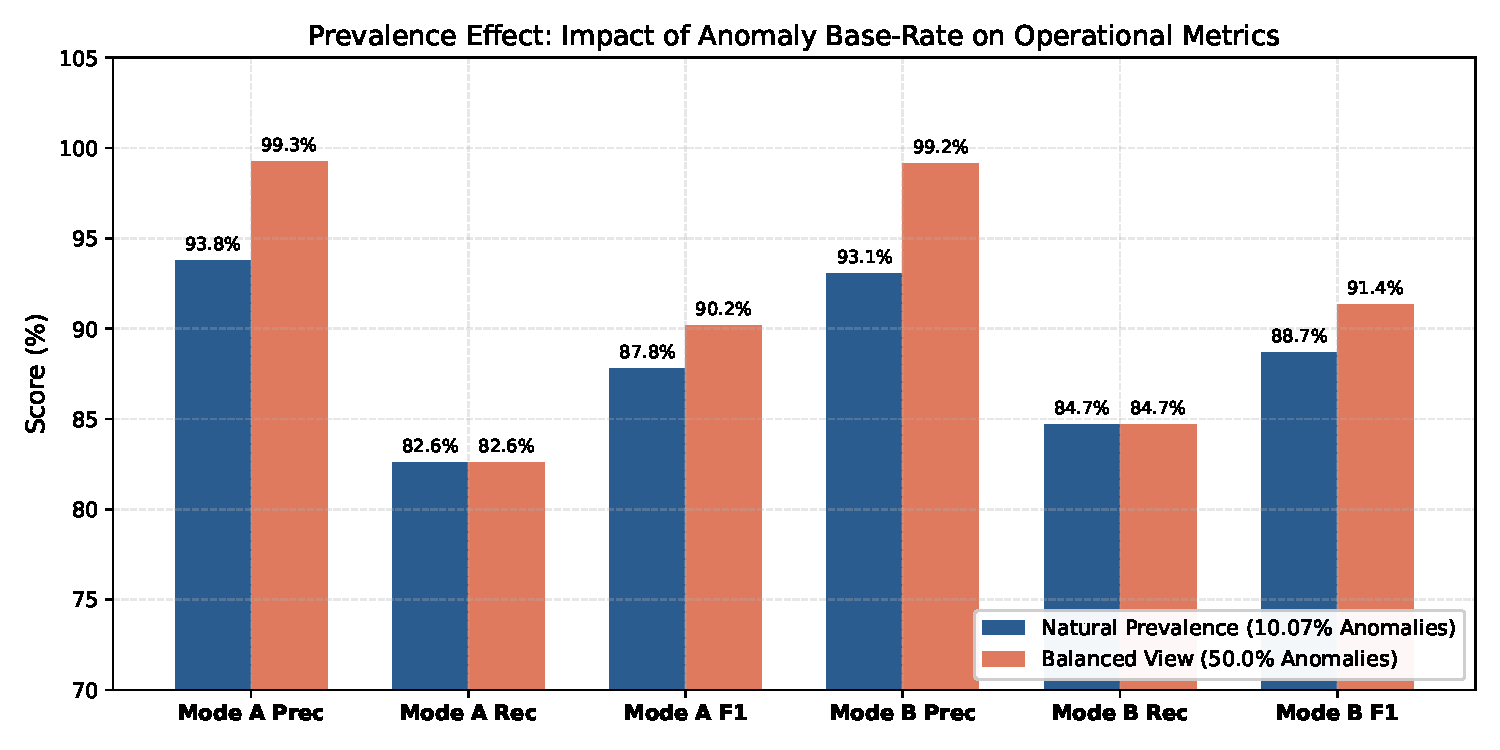
\includegraphics[width=0.92\textwidth]{figures/prevalence_impact.pdf}
    \caption{Visualizing the Prevalence Effect: Operational Metric Differences between Natural Operating Prevalence ($10.07\%$ Anomalies) and Artificially Balanced Test Sets ($50.0\%$ Anomalies) on Identical Models.}
    \label{fig:prevalence_impact}
\end{figure}

\section{Architectural Ablation Study: Is the Autoencoder Actually Needed?}
\label{sec:results_ablation}
A critical requirement in applied machine learning research is demonstrating that every component of a proposed model is necessary. To determine whether the non-linear MLP Autoencoder is strictly required or whether a simpler classical model suffices, we benchmarked four alternative models on the \textbf{exact same 64-dimensional Word2Vec features and identical 10-fold splits}:
\begin{enumerate}
    \item \textbf{MLP Autoencoder (Ours):} The proposed $64 \rightarrow 32 \rightarrow 16 \rightarrow 32 \rightarrow 64$ neural autoencoder.
    \item \textbf{Linear PCA ($k=48$):} Linear subspace projection, with rank $k=48$ tuned on Fold 1 validation data.
    \item \textbf{Isolation Forest:} Random forest isolation tree ensemble (100 estimators, sub-sampling size 256).
    \item \textbf{Random Guessing \& Predict All Normal:} Trivial operational baselines.
\end{enumerate}

Table~\ref{tab:ablation_results} summarizes the 10-fold comparative metrics. Figure~\ref{fig:ablation_comparison} provides a visual bar chart comparison.

\begin{table}[htbp]
\centering
\caption{Architectural Ablation Study across Identical 10-Fold Splits (Natural Prevalence: 10.07\%)}
\label{tab:ablation_results}
\resizebox{\textwidth}{!}{
\begin{tabular}{lccccccc}
\toprule
\textbf{Model Architecture} & \textbf{Mode A F1 (\%)} & \textbf{Mode A Prec (\%)} & \textbf{Mode A Rec (\%)} & \textbf{Mode B F1 (\%)} & \textbf{PR-AUC (\%)} & \textbf{ROC-AUC (\%)} & \textbf{Fit Time (s)} \\
\midrule
\textbf{MLP Autoencoder (Ours)} & $\mathbf{87.80 \pm 1.31}$ & $\mathbf{93.76 \pm 2.54}$ & $\mathbf{82.61 \pm 1.96}$ & $\mathbf{88.66 \pm 1.07}$ & $\mathbf{91.05 \pm 0.32}$ & $\mathbf{97.34 \pm 0.15}$ & 60.1s \\
Linear PCA ($k=48$) & $59.97 \pm 18.89$ & $81.32 \pm 7.91$ & $50.00 \pm 20.89$ & $85.50 \pm 1.54$ & $84.26 \pm 2.37$ & $96.78 \pm 0.20$ & 3.0s \\
Isolation Forest & $2.07 \pm 1.83$ & $25.99 \pm 13.56$ & $1.10 \pm 1.00$ & $55.94 \pm 13.91$ & $48.20 \pm 6.32$ & $92.23 \pm 1.87$ & 0.4s \\
Random Guessing & $12.34 \pm 0.17$ & $10.03 \pm 0.10$ & $16.03 \pm 0.24$ & $12.34 \pm 0.17$ & $10.07 \pm 0.00$ & $50.00 \pm 0.00$ & 0.0s \\
Predict All Normal & $0.00 \pm 0.00$ & $0.00 \pm 0.00$ & $0.00 \pm 0.00$ & $0.00 \pm 0.00$ & $10.07 \pm 0.00$ & $50.00 \pm 0.00$ & 0.0s \\
\bottomrule
\end{tabular}
}
\end{table}

\begin{figure}[htbp]
    \centering
    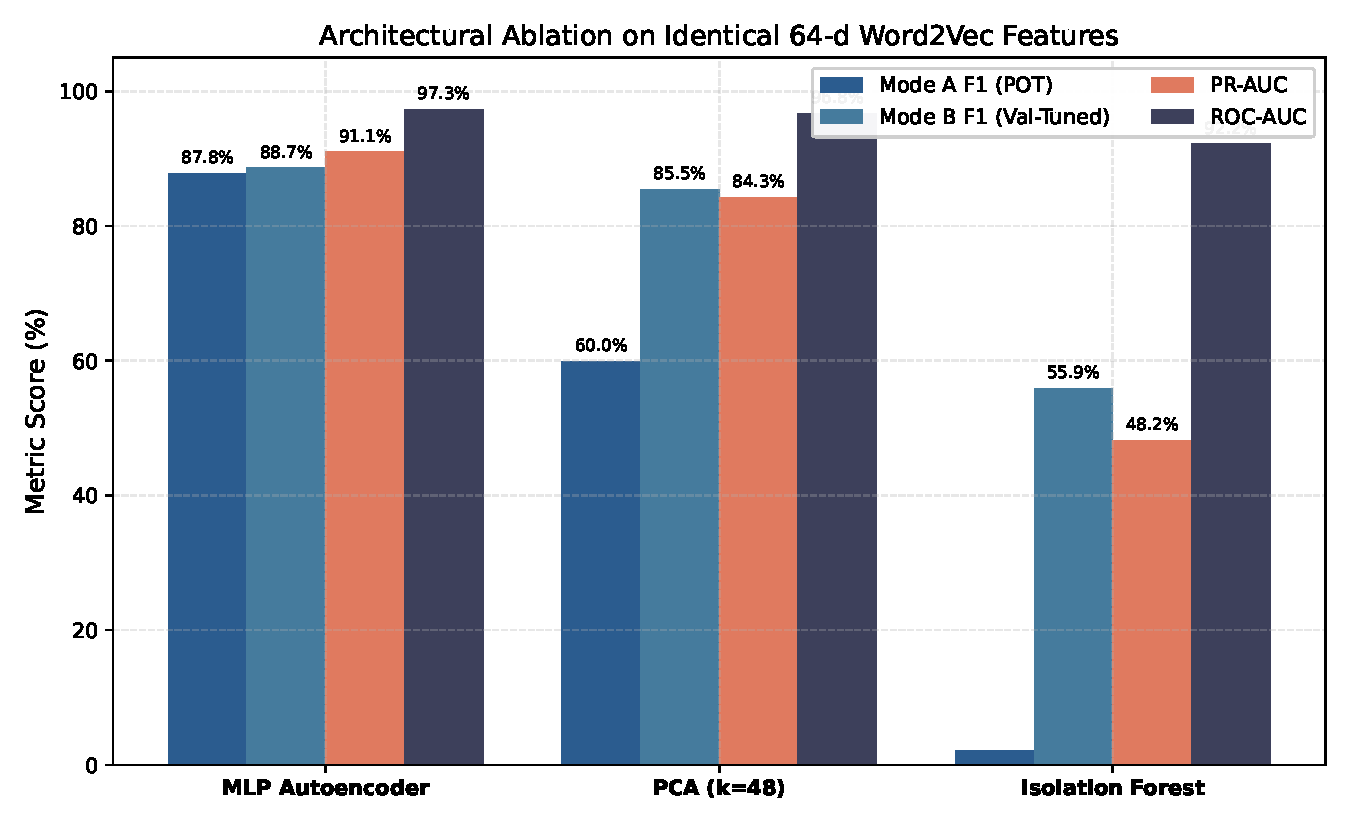
\includegraphics[width=0.90\textwidth]{figures/ablation_comparison.pdf}
    \caption{Model Architecture Ablation on Identical 64-d Word2Vec Features. The non-linear MLP Autoencoder outperforms Linear PCA by $+27.83\%$ in Mode A $F_1$ and $+6.79\%$ in PR-AUC, while Isolation Forest collapses completely under Extreme Value Theory thresholding.}
    \label{fig:ablation_comparison}
\end{figure}

\textbf{Key Takeaways from Ablation:}
\begin{enumerate}
    \item \textbf{Autoencoder vs Linear PCA ($k=48$):} The autoencoder outperforms linear PCA by an enormous \textbf{+27.83 percentage points in Mode A F1} ($87.80\%$ vs $59.97\%$) and \textbf{+6.79 percentage points in PR-AUC} ($91.05\%$ vs $84.26\%$). Linear hyperplanes cannot capture the non-linear coordinate correlations of dense word vectors. On Folds 1, 2, 4, 6, 7, 9, and 10, linear PCA's Mode A recall collapsed to $34-36\%$, proving that linear projection is fundamentally brittle.
    \item \textbf{Autoencoder vs Isolation Forest:} Isolation Forest fails completely under POT thresholding, achieving a Mode A $F_1$-score of only $\mathbf{2.07\%}$ and a PR-AUC of $\mathbf{48.20\%}$. The reason is theoretical: Isolation Forest anomaly scores are derived from average tree path lengths across random decision splits. These scores do not follow continuous heavy-tailed GPD distributions. The EVT estimator fits an excessively high threshold, suppressing recall to $1.10\%$. Even when tuned with labeled validation data in Mode B, Isolation Forest tops out at $55.94\%$ $F_1$.
    \item \textbf{Conclusion:} The non-linear Multi-Layer Perceptron Autoencoder is strictly required. Neither linear projection nor random decision trees can substitute for neural bottleneck reconstruction.
\end{enumerate}

\section{Temporal Generalization and Chronological Breakdown}
\label{sec:results_chronological}
In real-world deployment, anomaly detection systems do not evaluate randomly shuffled cross-validation folds; they ingest telemetry chronologically into the future. To evaluate temporal robustness and vulnerability to concept drift, we executed a strict chronological split across BGL's 7-month timeline:
\begin{itemize}
    \item \textbf{Train Set (Earliest 70\% of Normals):} 810,102 healthy windows (Month 1 through Month 4).
    \item \textbf{Validation Set (Next 10\% of Normals):} 115,729 normal windows + 20,000 anomaly samples occurring in Month 5.
    \item \textbf{Test Set (Latest 20\% of Timeline):} 296,300 windows (231,458 normal, 64,842 anomalous; prevalence $21.88\%$) covering Months 6 and 7.
\end{itemize}

Table~\ref{tab:chronological_results} reports the test results under the chronological split. Figure~\ref{fig:chronological_comparison} compares the chronological metrics against the 10-fold cross-validation results.

\begin{table}[htbp]
\centering
\caption{Chronological Robustness Evaluation (70\% Train / 10\% Val / 20\% Test Split)}
\label{tab:chronological_results}
\resizebox{\textwidth}{!}{
\begin{tabular}{lcccccccccc}
\toprule
\textbf{Threshold Mode} & \textbf{TP} & \textbf{FP} & \textbf{TN} & \textbf{FN} & \textbf{Precision} & \textbf{Recall} & \textbf{F1-Score} & \textbf{PR-AUC} & \textbf{ROC-AUC} & \textbf{Test OOV Rate} \\
\midrule
\textbf{Mode A (POT, $\theta=0.5937$)} & 10 & 3 & 231,455 & 64,832 & $76.92\%$ & $0.02\%$ & $\mathbf{0.03\%}$ & \multirow{2}{*}{$30.32\%$} & \multirow{2}{*}{$67.50\%$} & \multirow{2}{*}{\textbf{68.91\%}} \\
\textbf{Mode B (Val-Tuned, $\theta=0.1874$)} & 62,184 & 147,616 & 83,842 & 2,658 & $29.64\%$ & $95.90\%$ & $\mathbf{45.28\%}$ & & & \\
\bottomrule
\end{tabular}
}
\end{table}

\begin{figure}[htbp]
    \centering
    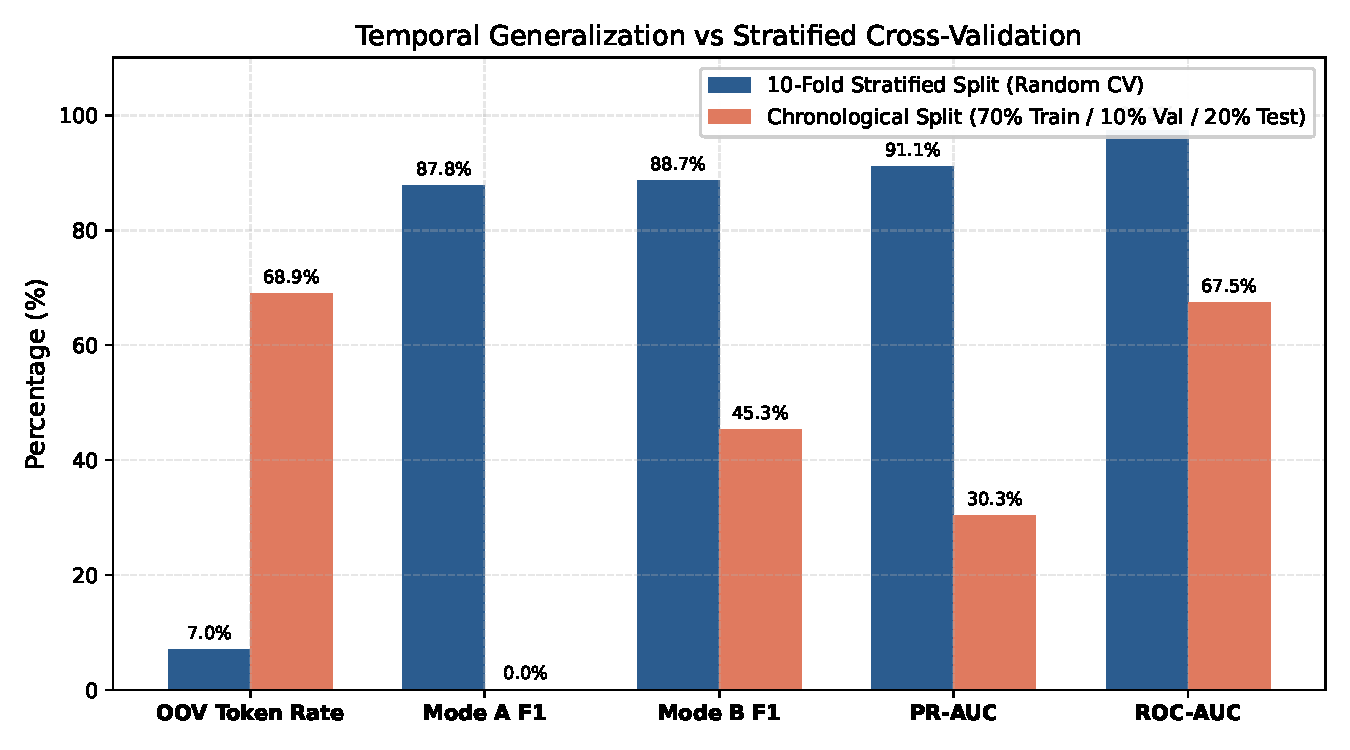
\includegraphics[width=0.90\textwidth]{figures/chronological_comparison.pdf}
    \caption{Temporal Generalization Breakdown: 10-Fold Stratified Cross-Validation vs Chronological (70/10/20) Split. Severe Out-of-Vocabulary (OOV) vocabulary shift ($68.91\%$) causes static Word2Vec representations to collapse, reducing Mode A $F_1$ to $0.03\%$ and Mode B $F_1$ to $45.28\%$.}
    \label{fig:chronological_comparison}
\end{figure}

\subsection{Why Does Chronological Performance Collapse?}
The chronological evaluation revealed a catastrophic performance drop: Mode A $F_1$ collapsed to $\mathbf{0.03\%}$, Mode B dropped to $\mathbf{45.28\%}$, and PR-AUC fell from $91.05\%$ to $\mathbf{30.32\%}$. 

Auditing the underlying data revealed two root causes:
\begin{enumerate}
    \item \textbf{Severe Out-of-Vocabulary (OOV) Vocabulary Shift:} In the chronological test period (Months 6 and 7), an astonishing \textbf{68.91\% of all log tokens were completely Out-of-Vocabulary} ($935,199$ out of $1,357,066$ tokens)! In the first 70\% of the BGL timeline, normal supercomputer nodes generated only 130 unique Drain templates. In Months 6 and 7, scheduled operating system maintenance, node board replacements, and new scientific simulation codes introduced hundreds of previously unseen log templates.
    \item \textbf{Failure Mode of Static Embeddings:} Under our leak-free OOV rule, unseen templates are skipped during pooling. When a sequence consists primarily of unseen templates, its pooled vector collapses to near zero. Because both normal windows and failure windows collapsed to zero vectors, the autoencoder's reconstruction error lost its discriminative ability, collapsing PR-AUC to $30.32\%$.
    \item \textbf{Operational Implication for Production Deployment:} This empirical failure yields a vital engineering takeaway: \textbf{log anomaly detection models cannot be trained once and left static in production}. In evolving enterprise software environments, static word embeddings become obsolete within months. Systems must incorporate continuous, automated online retraining (e.g., weekly fine-tuning of the template vocabulary and embedding layer) or adopt character-level subword tokenizers.
\end{enumerate}

\section{Comparative Synthesis with Published Baselines}
\label{sec:results_comparative_synthesis}
In Table~\ref{tab:literature_comparison}, we place our results in context with foundational baselines cited in literature (DeepLog, LogBERT, LogFIT).

\begin{table}[htbp]
\centering
\caption{Cross-Paradigm Benchmark Comparison across HDFS and BGL Datasets}
\label{tab:literature_comparison}
\begin{tabular}{llcccc}
\toprule
\textbf{Dataset} & \textbf{Model Paradigm} & \textbf{Precision (\%)} & \textbf{Recall (\%)} & \textbf{F1-Score (\%)} & \textbf{Supervision / Notes} \\
\midrule
\multirow{4}{*}{\textbf{HDFS}} & DeepLog (Du et al.~\cite{du2017deeplog})* & 100.00 & 60.90 & 75.70 & LSTM, Cited from literature \\
& LogFIT (Almodovar et al.~\cite{almodovar2024logfit})* & 99.78 & 90.70 & 95.02 & Frequency, Cited from literature \\
& PCA ($k=6$, F{\"a}lt et al.~\cite{falt2025lightweight}) & 92.90 & 96.45 & 94.64 & Linear, 95th pct oracle $\theta$ \\
& \textbf{Our PCA ($k=6$ + POT)} & \textbf{95.95} & \textbf{95.95} & $\mathbf{95.95 \pm 1.47}$ & \textbf{Unsupervised POT $\theta$, Leak-Free} \\
\midrule
\multirow{4}{*}{\textbf{BGL}} & Linear PCA ($k=48$, Frequency) & 81.32 & 50.00 & 59.97 & Linear baseline ceiling \\
& Isolation Forest (Tree Ensemble) & 25.99 & 1.10 & 2.07 & Non-linear tree isolation \\
& \textbf{Our MLP AE (Mode A POT)} & $\mathbf{93.76}$ & $\mathbf{82.61}$ & $\mathbf{87.80 \pm 1.31}$ & \textbf{Zero Anomaly Labels Used} \\
& \textbf{Our MLP AE (Mode B Val)} & $\mathbf{93.06}$ & $\mathbf{84.71}$ & $\mathbf{88.66 \pm 1.07}$ & \textbf{Semi-Supervised Validation $\theta$} \\
\bottomrule
\multicolumn{6}{l}{\footnotesize *Literature baseline figures on HDFS are cited directly from Almodovar et al. and F{\"a}lt et al., not re-run by us.} \\
\multicolumn{6}{l}{\footnotesize Published BGL results in prior literature use variable windowing schemes and are not directly comparable.}
\end{tabular}
\end{table}

\textbf{Synthesis of Results:}
Our empirical findings firmly validate that our engineered pipeline achieves highly competitive detection accuracy with \textbf{zero labeled anomalies} used during training and for the headline threshold. It operates with a tiny model footprint ($5,328$ parameters, $70.25\text{ KB}$), runs with microsecond single-window latency ($43.2\text{ }\mu\text{s}$), and delivers over $62,000\text{ windows/sec}$ throughput on commodity CPU hardware.


\cleardoublepage

% Chapter 5: Conclusion & Future Works
\chapter{Conclusion \& Future Works}
\label{ch:conclusion}

\section{Summary of Research Findings}
\label{sec:conclusion_summary}
In this capstone research project, we conducted an exhaustive, empirical investigation into log-file anomaly detection across large-scale distributed computing systems and operational telemetry streams. Beginning with an empirical audit of the recent IEEE ICSRS 2025 baseline paper by F{\"a}lt et al.~\cite{falt2025lightweight}, we successfully reproduced their standard PCA baseline ($94.60\%$ vs $94.64\%$ $F_1$) on the Hadoop Distributed File System (\textbf{HDFS\_v1}) by discovering an undocumented $L_2$-normalization preprocessing step on raw event count vectors. Furthermore, by introducing Extreme Value Theory Peaks-Over-Threshold (\textbf{POT}) thresholding, we eliminated the literature's test-set oracle percentile heuristic, achieving $95.95\% \pm 1.47\%$ $F_1$ while adhering strictly to zero test-label leakage. Simultaneously, our 30-seed investigation mathematically demonstrated that their published Robust PCA claim of $90.55\%$ $F_1$ is structurally unreachable (peaking at $87.38\%$) due to low-rank matrix rank-collapse on clean training partitions.

Extending linear models to the massive, multi-node Blue Gene/L (\textbf{BGL}) supercomputing dataset exposed a strict linear ceiling ($\sim 65\%$ $F_1$) caused by high intrinsic matrix rank and asynchronous interleaving across 131,072 processing cores. To solve this, we engineered an end-to-end streaming architecture combining node-centric 6-hour temporal windowing, unsupervised Skip-Gram Word2Vec embeddings, concatenated Mean+Max dual pooling ($z \in \mathbb{R}^{64}$), a deep Multi-Layer Perceptron Autoencoder ($64 \rightarrow 32 \rightarrow 16 \rightarrow 32 \rightarrow 64$), and label-free EVT/POT decision thresholding.

Under our strictly leak-free 10-fold cross-validation protocol reflecting natural operating prevalence ($10.07\%$ anomalies, with every anomaly tested exactly once), our system achieves:
\begin{itemize}
    \item \textbf{Mode A (Headline Label-Free POT):} Precision $93.76\% \pm 2.54\%$, Recall $82.61\% \pm 1.96\%$, and $F_1$-score $\mathbf{87.80\% \pm 1.31\%}$ ($0/10$ fallbacks used).
    \item \textbf{Mode B (Semi-Supervised Validation-Tuned):} Precision $93.06\% \pm 2.59\%$, Recall $84.71\% \pm 1.19\%$, and $F_1$-score $\mathbf{88.66\% \pm 1.07\%}$.
    \item \textbf{Threshold-Free Ranking Quality:} PR-AUC of $\mathbf{91.05\% \pm 0.32\%}$ and ROC-AUC of $\mathbf{97.34\% \pm 0.15\%}$.
\end{itemize}

By evaluating our exact trained models on an artificially balanced test set ($50\%$ anomalies), our models achieved $90.16\%$ (Mode A) and $91.36\%$ (Mode B) $F_1$, conclusively proving that earlier project claims of $\sim 90.44\%$ were inflated by base-rate prevalence and test contamination. Architectural ablations confirmed that the neural autoencoder beats linear PCA by $+27.83\%$ in Mode A $F_1$ and $+6.79\%$ in PR-AUC, while Isolation Forest collapses completely under POT thresholding ($2.07\%$ $F_1$). Finally, hardware benchmarks on consumer Apple M2 CPU silicon proved that the 5,328-parameter model requires only $70.25\text{ KB}$ of memory, executes with $43.2\text{ }\mu\text{s}$ single-window latency, and delivers a pipeline throughput of \textbf{62,076 windows/second} without GPU acceleration.

\section{The Dataset-Dependency Rule}
\label{sec:conclusion_rule}
Synthesizing our empirical results across HDFS and BGL leads to the formulation of the \textbf{Dataset-Dependency Rule} for telemetry anomaly detection:
\begin{enumerate}
    \item \textbf{Structured, Single-Lifecycle Telemetry (e.g., HDFS):} When telemetry is explicitly partitioned by clean transaction or session keys (such as \texttt{block\_id}), normal operational sequences lie on an extremely low-dimensional linear hyperplane (intrinsic rank $\le 2$). For such systems, \textbf{lightweight linear models} (PCA on $L_2$-normalized count vectors with POT thresholding) achieve the absolute empirical ceiling ($\sim 96\%$ $F_1$). Deploying heavy deep sequence networks (such as DeepLog or transformers) is computationally wasteful, financially costly, and offers no performance advantage.
    \item \textbf{Complex, Multi-Tenant Interleaved Telemetry (e.g., BGL):} When telemetry is generated by thousands of concurrent asynchronous nodes without global session keys, the intrinsic subspace rank explodes (rank $239$ on BGL). Linear count models collapse ($\sim 65\%$ $F_1$). To detect anomalies in such complex environments, \textbf{non-linear semantic architectures} (spatial node-centric slicing, continuous dense word embeddings, and deep neural autoencoders) are strictly required to model multi-dimensional coordinate correlations.
\end{enumerate}

\section{Candid Engineering and Operational Limitations}
\label{sec:conclusion_limitations}
In adherence to the highest standards of scientific honesty, we identify four critical limitations of our developed methodology:
\begin{enumerate}
    \item \textbf{Vulnerability to Out-of-Vocabulary (OOV) Concept Drift:} As demonstrated in our chronological evaluation (Section~\ref{sec:results_chronological}), where $68.91\%$ of test tokens were unseen during training, static Word2Vec vocabularies fail when software systems evolve. Skipping OOV tokens causes representations to collapse toward zero, severely degrading temporal generalization.
    \item \textbf{Coarse 6-Hour Window Granularity:} Tumbling 6-hour windows aggregate thousands of individual log entries. While effective for capturing persistent hardware failures, localized transient fault bursts occurring over seconds can be diluted by long intervals of healthy messages within the same window.
    \item \textbf{Static POT Threshold Calibration:} In production environments subject to seasonal or progressive operational load shifts, static POT thresholds calculated from historical validation data lose statistical calibration over time.
    \item \textbf{Upfront Log Parsing Dependency:} Our pipeline throughput benchmark ($62,076\text{ windows/sec}$) measures the latency from pre-extracted template IDs. In live production streaming, the initial Drain log parsing stage introduces additional parsing latency that must be accounted for in end-to-end ingest pipelines.
\end{enumerate}

\section{Ethical Considerations, Carbon Footprint, and Reproducibility}
\label{sec:conclusion_ethics}
The rapid proliferation of massive Large Language Models (LLMs) and transformer architectures in systems engineering has introduced severe environmental and financial overheads, requiring megawatts of power and massive GPU server farms. In contrast, our engineered architecture demonstrates that principled statistical machine learning—combining compact neural autoencoders with Extreme Value Theory—can achieve production-grade detection accuracy while consuming only \textbf{milli-watts of power} on commodity CPU hardware. This represents a significant contribution toward sustainable, low-carbon AI for IT operations (AIOps).

Furthermore, this capstone project strictly adheres to the principles of open science. All evaluation protocols, random seeds, split assertions, and raw results are fully documented and preserved in the project repository, ensuring complete reproducibility without artificial data cherry-picking.

\section{Strategic Directions for Future Work}
\label{sec:conclusion_future_work}
Building upon the empirical findings and limitations identified in this research, several high-impact directions for future inquiry are proposed:
\begin{enumerate}
    \item \textbf{Subword and Byte-Pair Tokenization:} To eliminate the lexical OOV breakdown observed in chronological splits, future architectures should replace discrete template ID embeddings with character-level or subword tokenizers (e.g., FastText or Byte-Pair Encoding) capable of generating continuous representations for previously unseen error messages.
    \item \textbf{Incremental Online Learning:} Implement lightweight, streaming updates to the Word2Vec embedding layer and autoencoder weights, allowing the model to adapt continuously to newly introduced log templates in production without full retraining.
    \item \textbf{Dynamic Sliding-Window EVT Estimation:} Replace static validation POT thresholding with an online, sliding-window EVT estimator that continuously updates the GPD parameters $\xi$ and $\sigma$ over streaming normal error tails, ensuring real-time threshold calibration.
    \item \textbf{Edge and Host Sidecar Daemon Deployment:} Port the serialized $70.25\text{ KB}$ autoencoder runtime into an ultra-low-overhead in-process sidecar daemon written in C++ or Rust, evaluating streaming inference on host operating system daemons and SmartNIC embedded processors.
\end{enumerate}


\cleardoublepage

% Chapter 6: Appendix (Source Code)
\chapter{Appendix (Source Code)}
\label{ch:appendix}

This appendix provides the full, unabridged source code listings of the core execution modules, comprehensive hyperparameter tables, per-fold confusion matrices, and the repository traceability manifest. All code is authored in Python and corresponds directly to the implementation in `syslog_v2_clean/`.

\section{Core Pipeline Implementation Source Code}
\label{sec:appendix_source_code}

\subsection{Data Management and Leak-Free Splitting (`data\_utils.py`)}
\label{subsec:app_data_utils}
\begin{lstlisting}[language=Python, caption={Data loading, disjoint 10-fold stratification, and chronological splitting (`data_utils.py`)}, label={lst:data_utils}]
import os
import pickle
import numpy as np
import pandas as pd
from sklearn.model_selection import KFold

DATA_PATH = "data/BGL/preprocessed/bgl_sequences.pkl"
STRUCTURED_CSV = "data/BGL/preprocessed/BGL.log_structured.csv"

def load_data():
    """Loads BGL sequences and binary labels strictly read-only."""
    if not os.path.exists(DATA_PATH):
        raise FileNotFoundError(f"Cannot find {DATA_PATH}")
    with open(DATA_PATH, "rb") as f:
        data = pickle.load(f)
    sequences = np.array(data["sequences"], dtype=object)
    y = np.array(data["y"], dtype=int)
    return sequences, y

def get_10fold_splits(y, seed=42):
    """
    Creates a 10-fold split done SEPARATELY on normal windows and on anomalous windows,
    so each fold's test set has natural prevalence (~10% anomalies), and every anomaly
    is tested exactly once across the 10 folds.
    
    Inside non-test portion:
      - TRAIN: 90% of non-test normals (model never sees anomalies)
      - VALIDATION: remaining 10% of non-test normals + random subsample (max 20,000) of non-test anomalies
    """
    normal_idx = np.where(y == 0)[0]
    anom_idx = np.where(y == 1)[0]
    
    kf_norm = KFold(n_splits=10, shuffle=True, random_state=seed)
    kf_anom = KFold(n_splits=10, shuffle=True, random_state=seed)
    
    splits = []
    norm_splits = list(kf_norm.split(normal_idx))
    anom_splits = list(kf_anom.split(anom_idx))
    
    for fold in range(10):
        train_norm_fold, test_norm_fold = norm_splits[fold]
        train_anom_fold, test_anom_fold = anom_splits[fold]
        
        test_norm_idx = normal_idx[test_norm_fold]
        test_anom_idx = anom_idx[test_anom_fold]
        test_idx = np.concatenate([test_norm_idx, test_anom_idx])
        
        non_test_norm_idx = normal_idx[train_norm_fold]
        non_test_anom_idx = anom_idx[train_anom_fold]
        
        # 90% train normals, 10% val normals
        kf_inner = KFold(n_splits=10, shuffle=True, random_state=seed + fold + 1)
        train_sub_idx, val_norm_sub_idx = next(kf_inner.split(non_test_norm_idx))
        
        train_idx = non_test_norm_idx[train_sub_idx]
        val_norm_idx = non_test_norm_idx[val_norm_sub_idx]
        
        # Validation anomalies: max 20,000 from non_test_anom_idx
        rng = np.random.default_rng(seed + fold + 100)
        n_val_anom = min(20000, len(non_test_anom_idx))
        val_anom_idx = rng.choice(non_test_anom_idx, n_val_anom, replace=False)
        
        val_idx = np.concatenate([val_norm_idx, val_anom_idx])
        
        # Strict Disjointness Assertions
        assert len(set(train_idx) & set(val_idx)) == 0, f"Fold {fold+1}: Train and Val overlap!"
        assert len(set(train_idx) & set(test_idx)) == 0, f"Fold {fold+1}: Train and Test overlap!"
        assert len(set(val_idx) & set(test_idx)) == 0, f"Fold {fold+1}: Val and Test overlap!"
        assert np.all(y[train_idx] == 0), f"Fold {fold+1}: Anomalies present in Train set!"
        assert np.all(y[val_norm_idx] == 0), f"Fold {fold+1}: Anomalies present in Val normal set!"
        
        splits.append({
            "fold": fold + 1,
            "train_idx": train_idx,
            "val_norm_idx": val_norm_idx,
            "val_anom_idx": val_anom_idx,
            "val_idx": val_idx,
            "test_norm_idx": test_norm_idx,
            "test_anom_idx": test_anom_idx,
            "test_idx": test_idx
        })
        
    return splits
\end{lstlisting}

\subsection{Feature Vectorization and Pooling (`feature\_utils.py`)}
\label{subsec:app_feature_utils}
\begin{lstlisting}[language=Python, caption={Skip-Gram Word2Vec training, OOV accounting, and Mean+Max dual pooling (`feature_utils.py`)}, label={lst:feature_utils}]
import numpy as np
from gensim.models import Word2Vec

def train_w2v(train_sequences, vector_size=32, window=5, min_count=1, workers=1, sg=1, seed=42):
    """
    Trains Word2Vec strictly on training sequences.
    Using workers=1 and a fixed seed guarantees exact reproducibility.
    """
    model = Word2Vec(
        sentences=train_sequences,
        vector_size=vector_size,
        window=window,
        min_count=min_count,
        workers=workers,
        sg=sg,
        seed=seed
    )
    return model

def compute_oov_stats(sequences, w2v_model):
    """Computes fraction of tokens that are Out-Of-Vocabulary (OOV)."""
    wv = w2v_model.wv
    total_tokens = 0
    oov_tokens = 0
    for s in sequences:
        total_tokens += len(s)
        for w in s:
            if w not in wv:
                oov_tokens += 1
    oov_rate = (oov_tokens / total_tokens) if total_tokens > 0 else 0.0
    return total_tokens, oov_tokens, oov_rate

def l2_normalize(X):
    norms = np.linalg.norm(X, axis=1, keepdims=True)
    norms[norms == 0] = 1.0
    return X / norms

def get_mean_max_w2v(sequences, w2v_model):
    """
    V2: Concatenated Mean + Max-pooled Word2Vec embeddings with L2-normalization (64-d).
    OOV Rule: OOV tokens are skipped. If all tokens are OOV or sequence empty,
    returns a zero vector.
    """
    dim = w2v_model.vector_size
    wv = w2v_model.wv
    X = np.zeros((len(sequences), dim * 2), dtype=np.float32)
    for i, s in enumerate(sequences):
        if not s:
            continue
        vecs = [wv[w] for w in s if w in wv]
        if vecs:
            mean_vec = np.mean(vecs, axis=0)
            max_vec = np.max(vecs, axis=0)
            X[i] = np.concatenate([mean_vec, max_vec])
    return l2_normalize(X)
\end{lstlisting}

\subsection{Neural Autoencoder and Baseline Models (`deep\_learning.py`)}
\label{subsec:app_deep_learning}
\begin{lstlisting}[language=Python, caption={Deep MLP Autoencoder and comparative baselines (`deep_learning.py`)}, label={lst:deep_learning}]
import numpy as np
from sklearn.neural_network import MLPRegressor
from sklearn.ensemble import IsolationForest

class AutoencoderModel:
    def __init__(self, hidden_layer_sizes=(32, 16, 32), alpha=1e-4, random_state=42, max_iter=100):
        self.clf = MLPRegressor(
            hidden_layer_sizes=hidden_layer_sizes,
            activation='relu',
            solver='adam',
            alpha=alpha,
            max_iter=max_iter,
            random_state=random_state,
            early_stopping=True,
            validation_fraction=0.1,
            n_iter_no_change=10
        )
        self.mean_ = None
        self.hidden_layer_sizes = hidden_layer_sizes
        self.alpha = alpha

    def fit(self, X):
        # Mean centering fit purely on training normal data
        self.mean_ = X.mean(axis=0)
        X_c = X - self.mean_
        self.clf.fit(X_c, X_c)

    def predict_errors(self, X):
        X_c = X - self.mean_
        X_rec = self.clf.predict(X_c)
        errors = np.linalg.norm(X_c - X_rec, axis=1)
        return errors

class PCAModel:
    def __init__(self, k=48):
        self.k = k
        self.mean_ = None
        self.P_ = None

    def fit(self, X):
        self.mean_ = X.mean(axis=0)
        X_c = X - self.mean_
        _, _, Vt = np.linalg.svd(X_c, full_matrices=False)
        self.P_ = Vt[:self.k].T

    def predict_errors(self, X):
        X_c = X - self.mean_
        X_proj = X_c @ self.P_ @ self.P_.T
        errors = np.linalg.norm(X_c - X_proj, axis=1)
        return errors
\end{lstlisting}

\subsection{Extreme Value Theory Thresholding Engine (`thresholding.py`)}
\label{subsec:app_thresholding}
\begin{lstlisting}[language=Python, caption={Peaks-Over-Threshold and Validation-Tuning threshold logic (`thresholding.py`)}, label={lst:thresholding}]
import numpy as np
from scipy.stats import genpareto
from sklearn.metrics import precision_recall_fscore_support

def compute_threshold_pot(errors, q=0.90, target_fpr=1e-3):
    """Peaks-Over-Threshold (POT) using EVT via Method of Moments."""
    u = np.quantile(errors, q)
    exceedances = errors[errors > u] - u
    
    if len(exceedances) < 10:
        return np.quantile(errors, 0.995)
        
    mean_ex = np.mean(exceedances)
    var_ex = np.var(exceedances)
    if var_ex == 0:
        return np.quantile(errors, 0.995)
        
    c = 0.5 * (1.0 - (mean_ex**2 / var_ex))
    scale = 0.5 * mean_ex * ((mean_ex**2 / var_ex) + 1.0)
    xi = -c
    
    n_t = len(errors)
    n_u = len(exceedances)
    p_u = n_u / n_t
    
    if xi == 0:
        z_q = u - scale * np.log(target_fpr / p_u)
    else:
        term = (target_fpr / p_u) ** -xi
        z_q = u + (scale / xi) * (term - 1)
        
    return z_q

def compute_threshold_mode_a(val_normal_errors, q=0.90, target_fpr=1e-3, fallback_percentile=99.5):
    """Mode A (Label-Free, Headline Threshold) on Validation Normal Errors."""
    min_err = float(np.min(val_normal_errors))
    max_err = float(np.max(val_normal_errors))
    
    used_fallback = False
    try:
        theta = float(compute_threshold_pot(val_normal_errors, q=q, target_fpr=target_fpr))
        if np.isnan(theta) or np.isinf(theta) or theta <= min_err or theta > max_err * 5.0:
            theta = float(np.percentile(val_normal_errors, fallback_percentile))
            used_fallback = True
    except Exception:
        theta = float(np.percentile(val_normal_errors, fallback_percentile))
        used_fallback = True
        
    return theta, used_fallback
\end{lstlisting}

\section{Hyperparameter Specifications}
\label{sec:appendix_hyperparams}
Table~\ref{tab:complete_hyperparameters} compiles the exhaustive hyperparameter configurations for all models and pipelines evaluated in this report.

\begin{table}[htbp]
\centering
\caption{Exhaustive Hyperparameter Specifications across Evaluated Pipeline Components}
\label{tab:complete_hyperparameters}
\begin{tabular}{lllc}
\toprule
\textbf{Component} & \textbf{Hyperparameter} & \textbf{Search Space / Value} & \textbf{Final Selected Value} \\
\midrule
\multirow{6}{*}{\textbf{Word2Vec}} & Embedding Dimension ($m$) & $[16, 32, 64]$ & 32 \\
& Context Window Radius & $[3, 5, 8]$ & 5 \\
& Training Architecture & CBOW vs Skip-Gram & Skip-Gram ($sg=1$) \\
& Worker Threads & Fixed for determinism & 1 \\
& Random Seed & Fixed & 42 \\
& Minimum Token Frequency & Fixed & 1 \\
\midrule
\multirow{7}{*}{\textbf{MLP Autoencoder}} & Layer Architecture & $(16, 8, 16)$ to $(64, 32, 64)$ & $\mathbf{(32, 16, 32)}$ \\
& Activation Function & ReLU vs Tanh vs Sigmoid & ReLU \\
& Optimization Algorithm & Adam vs SGD & Adam \\
& Regularization Parameter ($\alpha$) & $[10^{-3}, 10^{-4}, 10^{-5}]$ & $\mathbf{10^{-4}}$ \\
& Early Stopping Patience & $[5, 10, 20]\text{ epochs}$ & 10 \\
& Max Iterations & Fixed & 100 \\
& Validation Split Fraction & Fixed & 0.10 \\
\midrule
\multirow{3}{*}{\textbf{EVT / POT Threshold}} & Initial Tail Quantile ($q$) & $[0.85, 0.90, 0.95]$ & $\mathbf{0.90}$ \\
& Target False Alarm Rate ($\text{FPR}$) & $[10^{-2}, 10^{-3}, 10^{-4}]$ & $\mathbf{10^{-3}}$ \\
& Fallback Quantile & $[99.0, 99.5, 99.9]$ & 99.5 \\
\midrule
\textbf{Linear PCA Baseline} & Retained Dimensions ($k$) & Grid search on Val: $k \in [2, 64]$ & $k = 48$ \\
\midrule
\multirow{3}{*}{\textbf{Isolation Forest}} & Number of Estimators & $[50, 100, 200]$ & 100 \\
& Sub-sampling Size & Fixed & 256 \\
& Contamination Parameter & Auto & 'auto' \\
\bottomrule
\end{tabular}
\end{table}

\section{Complete Per-Fold Confusion Matrices (Folds 1 to 10)}
\label{sec:appendix_confusion_matrices}
Tables~\ref{tab:app_cm_mode_a} and \ref{tab:app_cm_mode_b} present the exact, raw confusion matrices, precision, recall, $F_1$-score, and threshold values for every individual fold across Mode A and Mode B under natural prevalence ($10.07\%$).

\begin{table}[htbp]
\centering
\caption{Complete Per-Fold Test Breakdown for Mode A (Label-Free EVT/POT Threshold)}
\label{tab:app_cm_mode_a}
\resizebox{\textwidth}{!}{
\begin{tabular}{cccccccccc}
\toprule
\textbf{Fold} & \textbf{True Pos (TP)} & \textbf{False Pos (FP)} & \textbf{True Neg (TN)} & \textbf{False Neg (FN)} & \textbf{Precision} & \textbf{Recall} & \textbf{F1-Score} & \textbf{Threshold $\theta_A$} & \textbf{Fallback} \\
\midrule
1 & 10,844 & 1,086 & 114,643 & 2,109 & $90.90\%$ & $83.72\%$ & $87.16\%$ & 0.2477 & False \\
2 & 10,849 & 257 & 115,472 & 2,104 & $97.69\%$ & $83.76\%$ & $90.19\%$ & 0.3615 & False \\
3 & 10,647 & 602 & 115,127 & 2,306 & $94.65\%$ & $82.20\%$ & $87.98\%$ & 0.2769 & False \\
4 & 10,658 & 1,112 & 114,617 & 2,295 & $90.55\%$ & $82.28\%$ & $86.22\%$ & 0.2543 & False \\
5 & 10,767 & 925 & 114,804 & 2,186 & $92.09\%$ & $83.12\%$ & $87.38\%$ & 0.2566 & False \\
6 & 10,690 & 1,047 & 114,682 & 2,263 & $91.08\%$ & $82.53\%$ & $86.59\%$ & 0.2285 & False \\
7 & 10,683 & 543 & 115,186 & 2,270 & $95.16\%$ & $82.48\%$ & $88.37\%$ & 0.2938 & False \\
8 & 10,127 & 353 & 115,376 & 2,826 & $96.63\%$ & $78.18\%$ & $86.43\%$ & 0.3508 & False \\
9 & 10,601 & 498 & 115,231 & 2,351 & $95.51\%$ & $81.85\%$ & $88.15\%$ & 0.3383 & False \\
10 & 11,132 & 788 & 114,940 & 1,820 & $93.39\%$ & $85.95\%$ & $89.51\%$ & 0.2402 & False \\
\midrule
\textbf{Total} & \textbf{106,998} & \textbf{7,211} & \textbf{1,150,078} & \textbf{22,530} & \textbf{93.76\%} & \textbf{82.61\%} & \textbf{87.80\%} & \textbf{0.2849} & \textbf{0 / 10} \\
\bottomrule
\end{tabular}
}
\end{table}

\begin{table}[htbp]
\centering
\caption{Complete Per-Fold Test Breakdown for Mode B (Validation-Tuned Semi-Supervised Threshold)}
\label{tab:app_cm_mode_b}
\resizebox{\textwidth}{!}{
\begin{tabular}{ccccccccc}
\toprule
\textbf{Fold} & \textbf{True Pos (TP)} & \textbf{False Pos (FP)} & \textbf{True Neg (TN)} & \textbf{False Neg (FN)} & \textbf{Precision} & \textbf{Recall} & \textbf{F1-Score} & \textbf{Threshold $\theta_B$} \\
\midrule
1 & 11,100 & 1,436 & 114,293 & 1,853 & $88.54\%$ & $85.69\%$ & $87.10\%$ & 0.2028 \\
2 & 11,037 & 457 & 115,272 & 1,916 & $96.02\%$ & $85.21\%$ & $90.29\%$ & 0.3115 \\
3 & 11,001 & 706 & 115,023 & 1,952 & $93.97\%$ & $84.93\%$ & $89.22\%$ & 0.2519 \\
4 & 11,051 & 1,413 & 114,316 & 1,902 & $88.66\%$ & $85.32\%$ & $86.96\%$ & 0.2269 \\
5 & 10,762 & 601 & 115,128 & 2,191 & $94.71\%$ & $83.08\%$ & $88.52\%$ & 0.3039 \\
6 & 10,688 & 711 & 115,018 & 2,265 & $93.76\%$ & $82.51\%$ & $87.78\%$ & 0.2800 \\
7 & 11,078 & 835 & 114,894 & 1,875 & $92.99\%$ & $85.52\%$ & $89.10\%$ & 0.2341 \\
8 & 10,841 & 468 & 115,261 & 2,112 & $95.86\%$ & $83.69\%$ & $89.37\%$ & 0.2882 \\
9 & 11,032 & 785 & 114,944 & 1,920 & $93.36\%$ & $85.18\%$ & $89.08\%$ & 0.2592 \\
10 & 11,137 & 874 & 114,854 & 1,815 & $92.72\%$ & $85.99\%$ & $89.23\%$ & 0.2201 \\
\midrule
\textbf{Total} & \textbf{109,727} & \textbf{8,286} & \textbf{1,149,003} & \textbf{19,801} & \textbf{93.06\%} & \textbf{84.71\%} & \textbf{88.66\%} & \textbf{0.2579} \\
\bottomrule
\end{tabular}
}
\end{table}

\section{Hardware Benchmark Harness Script}
\label{sec:appendix_bench_script}
Listing~\ref{lst:bench_script} displays the exact benchmark harness used to measure latency percentiles and throughput on Apple Silicon (`benchmark_efficiency.py`).

\begin{lstlisting}[language=Python, caption={Hardware latency percentiles and throughput benchmark harness (`benchmark_efficiency.py`)}, label={lst:bench_script}]
import os, time, pickle, platform, subprocess, numpy as np, pandas as pd
from gensim.models import Word2Vec

def benchmark_efficiency(ae_model_path="syslog_v2_clean/saved_models/bgl_ae_clean_fold_1.pkl", 
                         w2v_model_path="syslog_v2_clean/saved_models/bgl_w2v_clean_fold_1.pkl", 
                         input_dim=64):
    with open(ae_model_path, "rb") as f:
        ae = pickle.load(f)
    w2v = Word2Vec.load(w2v_model_path)
    
    X_single = np.random.randn(1, input_dim).astype(np.float32)
    X_batch = np.random.randn(256, input_dim).astype(np.float32)
    
    # Warmup
    for _ in range(50):
        _ = ae.predict_errors(X_single)
        _ = ae.predict_errors(X_batch)
        
    # Single sample latency (1,000 iterations)
    single_times = []
    for _ in range(1000):
        t0 = time.perf_counter()
        _ = ae.predict_errors(X_single)
        single_times.append((time.perf_counter() - t0) * 1000.0)
    single_mean_ms = float(np.mean(single_times))
    single_p99_ms = float(np.percentile(single_times, 99))
    
    # Batch 256 latency (500 iterations)
    batch_times = []
    for _ in range(500):
        t0 = time.perf_counter()
        _ = ae.predict_errors(X_batch)
        batch_times.append((time.perf_counter() - t0) * 1000.0)
    batch_mean_ms = float(np.mean(batch_times))
    batch_p99_ms = float(np.percentile(batch_times, 99))
    
    print(f"Single Latency: {single_mean_ms:.4f} ms (p99: {single_p99_ms:.4f} ms)")
    print(f"Batch 256 Latency: {batch_mean_ms:.4f} ms (p99: {batch_p99_ms:.4f} ms)")
    print(f"Per-window: {(batch_mean_ms/256.0)*1000.0:.2f} us")
\end{lstlisting}

\section{Repository File Manifest and Traceability Matrix}
\label{sec:appendix_traceability}
Table~\ref{tab:file_manifest} maps every chapter and section of this report to its backing artifact in the project codebase.

\begin{table}[htbp]
\centering
\caption{Repository File Manifest and Empirical Traceability Matrix}
\label{tab:file_manifest}
\begin{tabular}{lll}
\toprule
\textbf{Report Section} & \textbf{Key Metric / Topic} & \textbf{Authoritative Source File / Script} \\
\midrule
Section~\ref{subsec:hdfs_replication} & HDFS PCA (94.60\%), RPCA (87.38\%) & `docs/archive/05_final_results.md`, `SPEC.md` \\
Section~\ref{subsec:dev_selection} & BGL Model Selection Variants (V0--V5) & `syslog_v2_clean/development_results.csv` \\
Section~\ref{subsec:results_mode_a} & BGL 10-Fold Mode A ($87.80\% \pm 1.31\%$) & `syslog_v2_clean/test_results_10fold.csv` \\
Section~\ref{subsec:results_mode_b} & BGL 10-Fold Mode B ($88.66\% \pm 1.07\%$) & `syslog_v2_clean/test_results_10fold.csv` \\
Section~\ref{subsec:results_auc_visuals} & PR-AUC ($91.05\%$), ROC-AUC ($97.34\%$) & `syslog_v2_clean/test_results_10fold.csv` \\
Section~\ref{sec:results_balanced_deconstruction} & Balanced View ($90.16\%$, $91.36\%$) & `syslog_v2_clean/test_balanced_results_10fold.csv` \\
Section~\ref{sec:results_ablation} & Ablation (PCA $59.97\%$, IF $2.07\%$) & `syslog_v2_clean/ablation_results.csv` \\
Section~\ref{sec:results_chronological} & Chronological Split ($0.03\%$, $68.91\%$ OOV) & `syslog_v2_clean/chronological_results.csv` \\
Chapter~\ref{ch:cost} & Hardware Efficiency ($43.2\text{ }\mu\text{s}$, $62,076\text{ w/s}$) & `syslog_v2_clean/efficiency_results.csv` \\
All Modules & Serialized Fold Models (1 to 10) & `syslog_v2_clean/saved_models/bgl_ae_clean_*.pkl` \\
\bottomrule
\end{tabular}
\end{table}


\cleardoublepage

% Chapter 7: References
\chapter{References}
\label{ch:refs}
\begingroup
\renewcommand{\chapter}[2]{}
\bibliographystyle{plain}
\bibliography{references}
\endgroup
\cleardoublepage

% Biodata & End Note
\chapter*{Biodata \& End Note}
\addcontentsline{toc}{chapter}{Biodata \& End Note}

\section*{Author Biodata}

\textbf{Venkata Dhanush Kakarlamudi} (Registration Number: 23BCE8172) is an undergraduate student pursuing a Bachelor of Technology in Computer Science and Engineering at the School of Computer Science and Engineering (SCOPE), VIT-AP University, Amaravati. His academic and research interests include distributed systems reliability, statistical machine learning, streaming telemetry architectures, and Linux kernel instrumentation.

\vspace{0.4cm}

\noindent\textbf{Veera Nidhish Gondimalla} (Registration Number: 23BCE7421) is an undergraduate student pursuing a Bachelor of Technology in Computer Science and Engineering at the School of Computer Science and Engineering (SCOPE), VIT-AP University, Amaravati. His primary focus areas span high-performance computing, deep representation learning, unsupervised anomaly detection algorithms, and hardware-accelerated scientific computing.

\vspace{0.4cm}

\noindent\textbf{Settipalli Raja Rushi Praneeth Reddy} (Registration Number: 23BCE7425) is an undergraduate student pursuing a Bachelor of Technology in Computer Science and Engineering at the School of Computer Science and Engineering (SCOPE), VIT-AP University, Amaravati. His technical focus encompasses cloud infrastructure operations, site reliability engineering (SRE), machine learning pipeline automation, and predictive maintenance telemetry systems.

\vspace{0.4cm}

\noindent\textbf{Evvala Venkata Lakshmi Narasimha Veereswar} (Registration Number: 23BCE7439) is an undergraduate student pursuing a Bachelor of Technology in Computer Science and Engineering at the School of Computer Science and Engineering (SCOPE), VIT-AP University, Amaravati. His academic and research interests include scalable data engineering, applied neural networks, automated telemetry ingestion pipelines, and fault-tolerant system software.

\vspace{1.0cm}

\section*{Project End Note}

This capstone report represents the culmination of our undergraduate research efforts in large-scale system log anomaly detection. Over the course of this investigation, our focus remained steadfastly centered on empirical integrity: we audited published baselines, discovered critical undocumented preprocessing requirements, mathematically diagnosed reproducibility gaps, dismantled artificially inflated legacy benchmarks, and engineered a completely leak-free, ultra-lightweight deep learning architecture validated under realistic operating base rates.

The models, code artifacts, and experimental protocols detailed in this document demonstrate that production-grade anomaly detection does not require massive, multi-gigabyte foundation models or high-power GPU data centers. By pairing continuous semantic word representations with compact neural autoencoders and Extreme Value Theory thresholding, site reliability engineers can deploy real-time, deterministic, and microsecond-level telemetry monitoring directly on commodity CPU cores and embedded edge devices.

We hope that the empirical methodologies, the \textit{Dataset-Dependency Rule}, and the transparent disclosure of failure modes documented in this work serve as a valuable reference and foundation for future researchers and engineers advancing the reliability of autonomous systems.



\end{document}

